% THIS IS SIGPROC-SP.TEX - VERSION 3.1
% WORKS WITH V3.2SP OF ACM_PROC_ARTICLE-SP.CLS
% APRIL 2009
%
% It is an example file showing how to use the 'acm_proc_article-sp.cls' V3.2SP
% LaTeX2e document class file for Conference Proceedings submissions.
% ----------------------------------------------------------------------------------------------------------------
% This .tex file (and associated .cls V3.2SP) *DOES NOT* produce:
%       1) The Permission Statement
%       2) The Conference (location) Info information
%       3) The Copyright Line with ACM data
%       4) Page numbering
% ---------------------------------------------------------------------------------------------------------------
% It is an example which *does* use the .bib file (from which the .bbl file
% is produced).
% REMEMBER HOWEVER: After having produced the .bbl file,
% and prior to final submission,
% you need to 'insert'  your .bbl file into your source .tex file so as to provide
% ONE 'self-contained' source file.
%
% Questions regarding SIGS should be sent to
% Adrienne Griscti ---> griscti@acm.org
%
% Questions/suggestions regarding the guidelines, .tex and .cls files, etc. to
% Gerald Murray ---> murray@hq.acm.org
%
% For tracking purposes - this is V3.1SP - APRIL 2009

\documentclass[conference]{IEEEtran}
\usepackage[ruled, vlined, nofillcomment, linesnumbered]{algorithm2e}
\usepackage{cite}
\usepackage{url}
\usepackage{amsmath}
\usepackage{amsthm}
\usepackage{amssymb}
\usepackage{numprint} 
%\usepackage{amsthm}
\usepackage{graphicx}
%\usepackage[tight]{subfigure}
\usepackage[english]{babel}
\usepackage{booktabs}
\usepackage{nicefrac}
\usepackage{verbatim}
\usepackage{float}
\usepackage{xspace}
\usepackage[table]{xcolor}
%\usepackage[font=bf,labelsep=space]{caption}
\usepackage[show]{notes}
\usepackage{flushend}


\usepackage{tikz}
\usetikzlibrary{positioning,calc}

\usepackage{pgfplots}


\usepackage{caption}
\usepackage{subcaption}



%% Data names
\newcommand{\dtname}[1]{\textsl{#1}}
\newcommand{\dolphins}{\dtname{dolphins}\xspace}
\newcommand{\karate}{\dtname{karate}\xspace}
\newcommand{\lesmis}{\dtname{lesmis}\xspace}
\newcommand{\astro}{\dtname{astro}\xspace}
\newcommand{\enron}{\dtname{enron}\xspace}
\newcommand{\facebook}{\dtname{facebook}\xspace}
\newcommand{\EUall}{\dtname{EUall}\xspace}
\newcommand{\dblp}{\dtname{dblp}\xspace}
\newcommand{\youtube}{\dtname{youtube}\xspace}
\newcommand{\roadnet}{\dtname{roadnet}\xspace}
\newcommand{\skitter}{\dtname{skitter}\xspace}

\newcommand{\exact}{\textsc{Exact}\xspace}
\newcommand{\hillclimb}{\textsc{Hill Climb}\xspace}
\newcommand{\kmeans}{\textsc{K-Means}\xspace}


\newtheorem{theorem}{Theorem}
\newtheorem{lemma}[theorem]{Lemma}
\newtheorem{proposition}[theorem]{Proposition}
\newtheorem{corollary}[theorem]{Corollary}
\newtheorem{definition}[theorem]{Definition}
\newtheorem{example}[theorem]{Example}
\newtheorem{problem}[theorem]{Problem}



\newcommand{\set}[1]{\left\{#1\right\}}
\newcommand{\pr}[1]{\left(#1\right)}
\newcommand{\fpr}[1]{\mathopen{}\left(#1\right)}
\newcommand{\spr}[1]{\left[#1\right]}
\newcommand{\fspr}[1]{\mathopen{}\left[#1\right]}
\newcommand{\brak}[1]{\left<#1\right>}
\newcommand{\abs}[1]{{\left|#1\right|}}
\newcommand{\norm}[1]{\left\|#1\right\|}
\newcommand{\enset}[2]{\left\{#1 ,\ldots , #2\right\}}
\newcommand{\enpr}[2]{\pr{#1 ,\ldots , #2}}
\newcommand{\enlst}[2]{{#1} ,\ldots , {#2}}
% \newcommand{\vect}[1]{\spr{#1}}
\newcommand{\vect}[1]{\mathbf{#1}}
\newcommand{\envec}[2]{\vect{#1 ,\ldots , #2}}
\newcommand{\real}{\mathbb{R}}
\newcommand{\np}{\textbf{NP}}
\newcommand{\poly}{\textbf{P}}
\newcommand{\naturals}{\mathbb{N}}
\newcommand{\funcdef}[3]{{#1}:{#2} \to {#3}}
\newcommand{\define}{\leftarrow}
\newcommand{\reals}{{\mathbb{R}}}
\newcommand{\dg}[1]{\dispfunc{\mathrm{deg}}{#1}}
\newcommand{\bigO}[1]{\dispfunc{\mathcal{O}}{#1}}
\newcommand{\role}{r}
\newcommand{\prof}[1]{\dispfunc{\vect{p}}{#1}}
\newcommand{\centroid}{\vect{c}}
\newcommand{\centroidcoord}{{c}}
\newcommand{\dist}[1]{\dispfunc{d}{#1}}
\newcommand{\elltwo}[1]{\dispfunc{\ell_2}{#1}}
\newcommand{\cost}[1]{\dispfunc{c}{#1}}
\newcommand{\gain}[1]{\dispfunc{\mathrm{gain}}{#1}}
\newcommand{\nbhdg}[1]{\dispfunc{\mathrm{ng}}{#1}}


\newcommand{\fm}[1]{{\mathcal{#1}}}

\DeclareRobustCommand{\dispfunc}[2]{%
	\ensuremath{%
		\ifthenelse{\equal{#2}{}}%
			{\mathit{#1}}%
			{\mathit{#1}\fpr{#2}}}}

\newcommand{\prbrm}{\textsc{Roles}\xspace}
\newcommand{\prbrmfixed}{\textsc{Roles-Fixed\-Centroids}\xspace}
\newcommand{\tmatch}{\textsc{3D-Matching}\xspace}
\newcommand{\tsat}{\textsc{3-Sat}\xspace}
\newcommand{\tuples}{\textsc{Tuples}\xspace}
\newcommand{\algperfect}{\textsc{Perfect}\xspace}
\newcommand{\alggreedy}{\textsc{Greedy}\xspace}
\newcommand{\algiterative}{\textsc{Iterative}\xspace}
\newcommand{\algcluster}{\textsc{Cluster}\xspace}
\newcommand{\algkm}{\textsc{itr}\xspace}
\newcommand{\algrolx}{\textsc{RolX}\xspace}

\newcommand{\alginitdeg}{\textsc{deg}\xspace}
\newcommand{\alginitrnd}{\textsc{rnd}\xspace}
\newcommand{\alginitone}{\textsc{one}\xspace}
\newcommand{\alginitkm}{\textsc{i+g}\xspace}

%% editing macros
\newcommand{\para}[1]{\noindent{\bf{#1}}}
\newcommand{\spara}[1]{\smallskip\noindent{\bf{#1}}}
\newcommand{\mpara}[1]{\medskip\noindent{\bf{#1}}}
\newcommand{\bpara}[1]{\bigskip\noindent{\bf{#1}}}


% PGF stuff

\pgfdeclarelayer{background}
\pgfdeclarelayer{foreground}
\pgfsetlayers{background,main,foreground}


\definecolor{yafaxiscolor}{rgb}{0.3, 0.3, 0.3}

\definecolor{yafcolor1}{rgb}{0.4, 0.165, 0.553}
\definecolor{yafcolor2}{rgb}{0.949, 0.482, 0.216}
\definecolor{yafcolor3}{rgb}{0.47, 0.549, 0.306}
\definecolor{yafcolor4}{rgb}{0.925, 0.165, 0.224}
\definecolor{yafcolor5}{rgb}{0.141, 0.345, 0.643}
\definecolor{yafcolor6}{rgb}{0.965, 0.933, 0.267}
\definecolor{yafcolor7}{rgb}{0.627, 0.118, 0.165}
\definecolor{yafcolor8}{rgb}{0.878, 0.475, 0.686}



\tikzstyle{graphedge} = [black, thick, opacity = 0.5, bend left = 10]
\tikzstyle{graphnode} = [circle, draw, line width = 1pt, text = black, inner sep = 0.5pt, text width = 7pt, align = center]
\tikzstyle{graphcl1} = [yafcolor1, fill = yafcolor1!10]
\tikzstyle{graphcl2} = [yafcolor3, fill = yafcolor3!10]
\tikzstyle{graphcl3} = [yafcolor2, fill = yafcolor2!10]







\newlength{\yafaxispad}
\setlength{\yafaxispad}{-4pt}
\newlength{\yaftlpad}
\setlength{\yaftlpad}{\yafaxispad}
\addtolength{\yaftlpad}{-0pt}
\newlength{\yaflabelpad}
\setlength{\yaflabelpad}{-2pt}
\newlength{\yafaxiswidth}
\setlength{\yafaxiswidth}{1.2pt}
\newlength{\yafticklen}
\setlength{\yafticklen}{2pt}

\makeatletter
\def\pgfplots@drawtickgridlines@INSTALLCLIP@onorientedsurf#1{}
\makeatother

\newcommand{\yafdrawxaxis}[2]{
	\pgfplotstransformcoordinatex{#1}\let\xmincoord=\pgfmathresult 
	\pgfplotstransformcoordinatex{#2}\let\xmaxcoord=\pgfmathresult 
	\pgfsetlinewidth{\yafaxiswidth} 
	\pgfsetcolor{yafaxiscolor}
	\pgfpathmoveto{\pgfpointadd{\pgfpointadd{\pgfplotspointrelaxisxy{0}{0}}{\pgfqpointxy{\xmincoord}{0}}}{\pgfqpoint{-0.5\yafaxiswidth}{\yafaxispad}}}
	\pgfpathlineto{\pgfpointadd{\pgfpointadd{\pgfplotspointrelaxisxy{0}{0}}{\pgfqpointxy{\xmaxcoord}{0}}}{\pgfqpoint{0.5\yafaxiswidth}{\yafaxispad}}}
	\pgfusepath{stroke}

}
\newcommand{\yafdrawyaxis}[2]{
	\pgfplotstransformcoordinatey{#1}\let\ymincoord=\pgfmathresult 
	\pgfplotstransformcoordinatey{#2}\let\ymaxcoord=\pgfmathresult 
	\pgfsetlinewidth{\yafaxiswidth} 
	\pgfsetcolor{yafaxiscolor}
	\pgfpathmoveto{\pgfpointadd{\pgfpointadd{\pgfplotspointrelaxisxy{0}{0}}{\pgfqpointxy{0}{\ymincoord}}}{\pgfqpoint{\yafaxispad}{-0.5\yafaxiswidth}}}
	\pgfpathlineto{\pgfpointadd{\pgfpointadd{\pgfplotspointrelaxisxy{0}{0}}{\pgfqpointxy{0}{\ymaxcoord}}}{\pgfqpoint{\yafaxispad}{0.5\yafaxiswidth}}}
	\pgfusepath{stroke}
}

\newcommand{\yafdrawaxis}[4]{\yafdrawxaxis{#1}{#2}\yafdrawyaxis{#3}{#4}}

\pgfplotscreateplotcyclelist{yaf}{% 
{yafcolor1,mark options={scale=0.75},mark=o}, 
{yafcolor2,mark options={scale=0.75},mark=square},
{yafcolor3,mark options={scale=0.75},mark=triangle},
{yafcolor4,mark options={scale=0.75},mark=o},
{yafcolor5,mark options={scale=0.75},mark=o},
{yafcolor6,mark options={scale=0.75},mark=o},
{yafcolor7,mark options={scale=0.75},mark=o},
{yafcolor8,mark options={scale=0.75},mark=o}} 

\pgfplotsset{axis y line=left, axis x line=bottom,
	tick align=outside,
	compat = 1.3,
	tickwidth=\yafticklen,
	clip = false,
	every axis title shift = 0pt,
    x axis line style= {-, line width = 0pt, opacity = 0},
    y axis line style= {-, line width = 0pt, opacity = 0},
    x tick style= {line width = \yafaxiswidth, color=yafaxiscolor, yshift = \yafaxispad},
    y tick style= {line width = \yafaxiswidth, color=yafaxiscolor, xshift = \yafaxispad},
    x tick label style = {font=\scriptsize, yshift = \yaftlpad},
    y tick label style = {font=\scriptsize, xshift = \yaftlpad},
    every axis y label/.style = {at = {(ticklabel cs:0.5)}, rotate=90, anchor=center, font=\scriptsize, yshift = -\yaflabelpad},
    every axis x label/.style = {at = {(ticklabel cs:0.5)}, anchor=center, font=\scriptsize, yshift = \yaflabelpad},
    x tick label style = {font=\scriptsize, yshift = 1pt},
    grid = major,
    major grid style  = {dash pattern = on 1pt off 3 pt},
	every axis plot post/.append style= {line width=\yafaxiswidth} ,
	legend cell align = left,
	legend style = {inner sep = 1pt, cells = {font=\scriptsize}},
	legend image code/.code={%
		\draw[mark repeat=2,mark phase=2,#1] 
		plot coordinates { (0cm,0cm) (0.15cm,0cm) (0.3cm,0cm) };% 
	} 
}


\renewcommand{\IEEEQED}{\IEEEQEDopen}

\begin{document}

\title{A combinatorial approach to role discovery}

% \title{Role-based role discovery}
%\subtitle{} 
%\titlenote{A full version of this paper is available as
%\textit{Author's Guide to Preparing ACM SIG Proceedings Using
%\LaTeX$2_\epsilon$\ and BibTeX} at
%\texttt{www.acm.org/eaddress.htm}}}
%
% You need the command \numberofauthors to handle the 'placement
% and alignment' of the authors beneath the title.
%
% For aesthetic reasons, we recommend 'three authors at a time'
% i.e. three 'name/affiliation blocks' be placed beneath the title.
%
% NOTE: You are NOT restricted in how many 'rows' of
% "name/affiliations" may appear. We just ask that you restrict
% the number of 'columns' to three.
%
% Because of the available 'opening page real-estate'
% we ask you to refrain from putting more than six authors
% (two rows with three columns) beneath the article title.
% More than six makes the first-page appear very cluttered indeed.
%
% Use the \alignauthor commands to handle the names
% and affiliations for an 'aesthetic maximum' of six authors.
% Add names, affiliations, addresses for
% the seventh etc. author(s) as the argument for the
% \additionalauthors command.
% These 'additional authors' will be output/set for you
% without further effort on your part as the last section in
% the body of your article BEFORE References or any Appendices.

%\numberofauthors{3} %  in this sample file, there are a *total*
% of EIGHT authors. SIX appear on the 'first-page' (for formatting
% reasons) and the remaining two appear in the \additionalauthors section.
%
%\author{
% You can go ahead and credit any number of authors here,
% e.g. one 'row of three' or two rows (consisting of one row of three
% and a second row of one, two or three).
%
% The command \alignauthor (no curly braces needed) should
% precede each author name, affiliation/snail-mail address and
% e-mail address. Additionally, tag each line of
% affiliation/address with \affaddr, and tag the
% e-mail address with \email.
%
% 1st. author
%\alignauthor A.Merlin Arockiasamy\\
%\affaddr Aalto University \\
%\affaddr Espoo, Finland \\
%\email{albert.arockiasamy@aalto.fi}
%\and
%\alignauthor Nikolaj Tatti \\
%\affaddr Aalto University and HIIT \\
%\affaddr Espoo, Finland \\
%\email{nikolaj.tatti@aalto.fi}
%\alignauthor Aristides Gionis \\
%\affaddr Aalto University and HIIT \\
%\documentclass{sig-alternate}
%\affaddr Espoo, Finland \\
%\email{aristides.gionis@aalto.fi}
%}

\author{Anonymized Authors}
\date{}


\maketitle

\begin{abstract} 

We provide a new formulation for the 
problem of role discovery in graphs. 
Our definition is structural and recursive: 
two vertices should be assigned to the same role
if the roles of their neighbors, when viewed as multi-sets, are similar enough.
An attractive characteristic of our approach 
is that it is based on optimizing a well-defined objective function, 
and thus, contrary to previous approaches, 
the role-discovery task can be studied with the tools of combinatorial optimization.

We demonstrate that, when fixing the number of roles to be used, 
the proposed role-discovery problem is \np-hard, 
while another (seemingly easier) version of the problem is \np-hard to approximate.
On the positive side, 
despite the recursive nature of our objective function, 
we can show that finding a \emph{perfect} (zero-cost) role assignment
with the minimum number of roles can be solved in polynomial time. 
We do this by connecting the zero-cost role assignment with the notion of equitable partition.
% Unfortunately, this polynomially-time solvable version of the problem
% is not very useful in practice, as the minimum number of roles found tends to be large.
For the more practical version of the problem with fixed number of roles
we present two natural heuristic methods, 
and discuss how make them scalable in large graphs.

\end{abstract}
% A category with the (minimum) three required fields
%\category{H.2.8}{Database Applications}{Data Mining}
%A category including the fourth, optional field follows...
%\category{E.1}{Data Structures}{Graphs and networks}

%\terms{Algorithms, Design, Performance, Experimentation}

%\keywords{Graph mining, role discovery}
\section{Introduction}


Modeling interconnected entities as graphs (or networks)
allows us study the global structure and function of a system,
instead of looking at single entities in isolation.
The understanding of the structure of a network in a holistic way
can be further supported by our ability to 
understand the \emph{role} of a single vertex 
with respect to its local neighborhood, 
or with respect to the whole network.
Accordingly, 
\emph{role discovery} 
has emerged as an important
graph-mining task~\cite{gilpin2013guided,danilevsky2013entity,henderson2012rolx,rossi2015role,ruan2014simultaneous,yang2015network,zhao2013inferring}, 
together with other standard graph-mining problems, 
such as community detection, link prediction,  etc.

Role discovery can be a valuable tool for exploratory graph mining. 
For instance, identifying the role of person in a social network 
may provide cues for understanding the social behavior of the person
in relation to her peers. 
Similarly, identifying the role of a vertex in a technological network 
may give useful information about the function of the vertex in the network, 
or it may be used to detect anomalies~\cite{rossi2013multi}.
Rossi and Ahmed~\cite{rossi2015role}
provide an extensive and well-documented list of graph-mining tasks
that can be facilitated by role discovery. 
The list includes applications such as 
classification, active learning, graph visualization, 
transfer learning, graph compression, entity resolution, and more.

% Not really needed, if we are low on space
%In general, role discovery can be seen as a process that
%partitions the vertices of a graph into equivalence classes.
%Nodes in the same class are assigned to the same role. 
%Equivalence classes are typically
%aiming at capturing the structural relation between the vertices and their neighbors. 
%In this way roles can represent 
%structural patterns in the graph, 
%such as, star centers, bridges, peripheral vertices, vertices in near-cliques, etc.~\cite{henderson2012rolx}.

Various approaches have been proposed
for defining when two vertices should be considered equivalent and, thus,  
should be assigned to the same role. 
Some of the first methods % proposed in mathematical sociology
rely on identifying structural or automorphic equivalence 
classes~\cite{everett1994regular,lorrain1971structural}, 
while newer methods 
represent vertices by feature vectors 
and assign to the same role vertices with similar 
feature vectors~\cite{henderson2012rolx,rossi2015role,rossi2013modeling,zhao2013inferring}.

\iffalse
An attractive definition for 
discovering roles in networks is based on the concept of
\emph{regular equivalence}~\cite{everett1994regular,white1983graph}:
According to regular equivalence, 
two vertices should be assigned to the same role
only if their neighbors have the same roles, ignoring multiplicities.
For example, 
for the collaboration network of a company
we may discover 
that vertices with role $A$ (``project manager'')
are connected to vertices with role 
$B$ (``business analyst'') and $C$ (``s/w developer''), 
while vertices with roles $B$ and $C$ are typically not connected to each other. 
\fi

In this paper we present a new approach to role discovery, 
inspired by the definition of \emph{equitable partition} of vertices.
A partition is equitable if the edges respect partition: 
two groups of vertices in equitable partition are either fully connected or fully disconnected.
As the original definition is too strict to be of use in real-world datasets, 
we introduce a \emph{relaxation} that provides robustness and can tolerate noise in the data.
In particular, we define an objective function that quantifies
the degree to which a given role assignment 
satisfies equitability.
Given a target number of roles $k$
we ask to find the role assignment that minimizes our objective function.
%Multiplicities are taken into account: a vertex with 100 neighbors having role $A$
%is treated differently than a vertex with a single neighbor having role $A$.

\begin{figure}
\begin{tikzpicture}[baseline = (current bounding box.south)]
\node[graphcl3, graphnode] (n0) at (-0.195230in, -0.629600in) {$\scriptscriptstyle 0$};
\node[graphcl2, graphnode] (n1) at (0.237355in, -0.458975in) {$\scriptscriptstyle 1$};
\node[graphcl2, graphnode] (n4) at (-0.202680in, -0.378515in) {$\scriptscriptstyle 4$};
\node[graphcl1, graphnode] (n3) at (0.055400in, -0.662550in) {$\scriptscriptstyle 3$};
\node[graphcl1, graphnode] (n5) at (-0.495860in, -0.631050in) {$\scriptscriptstyle 5$};
\node[graphcl1, graphnode] (n9) at (0.056340in, -0.331475in) {$\scriptscriptstyle 9$};
\node[graphcl1, graphnode] (n12) at (-0.627850in, -0.402875in) {$\scriptscriptstyle 12$};
\node[graphcl1, graphnode] (n17) at (-0.132200in, -0.855000in) {$\scriptscriptstyle 17$};
\node[graphcl1, graphnode] (n26) at (-0.429895in, -0.858850in) {$\scriptscriptstyle 26$};
\node[graphcl2, graphnode] (n2) at (0.192100in, -0.057610in) {$\scriptscriptstyle 2$};
\node[graphcl2, graphnode] (n13) at (0.446975in, -0.093245in) {$\scriptscriptstyle 13$};
\node[graphcl1, graphnode] (n20) at (0.481320in, -0.849000in) {$\scriptscriptstyle 20$};
\node[graphcl2, graphnode] (n6) at (-0.304685in, 0.139655in) {$\scriptscriptstyle 6$};
\node[graphcl3, graphnode] (n7) at (0.286355in, 0.318150in) {$\scriptscriptstyle 7$};
\node[graphcl2, graphnode] (n8) at (-0.172725in, 0.302300in) {$\scriptscriptstyle 8$};
\node[graphcl2, graphnode] (n18) at (-0.087970in, -0.095142in) {$\scriptscriptstyle 18$};
\node[graphcl1, graphnode] (n25) at (0.554350in, -0.342300in) {$\scriptscriptstyle 25$};
\node[graphcl1, graphnode] (n31) at (0.676500in, -0.012445in) {$\scriptscriptstyle 31$};
\node[graphcl2, graphnode] (n11) at (-0.570100in, 0.070990in) {$\scriptscriptstyle 11$};
\node[graphcl1, graphnode] (n23) at (-0.379895in, 0.573350in) {$\scriptscriptstyle 23$};
\node[graphcl1, graphnode] (n28) at (-0.455200in, -0.091015in) {$\scriptscriptstyle 28$};
\node[graphcl1, graphnode] (n32) at (-0.455200in, -0.291015in) {$\scriptscriptstyle 32$};
\node[graphcl1, graphnode] (n29) at (-0.528800in, 0.497080in) {$\scriptscriptstyle 29$};
\node[graphcl1, graphnode] (n19) at (0.578350in, 0.362865in) {$\scriptscriptstyle 19$};
\node[graphcl1, graphnode] (n14) at (0.681150in, 0.180865in) {$\scriptscriptstyle 14$};
\node[graphcl1, graphnode] (n22) at (0.257470in, 0.803250in) {$\scriptscriptstyle 22$};
\node[graphcl1, graphnode] (n15) at (0.574150in, 0.648200in) {$\scriptscriptstyle 15$};
\node[graphcl1, graphnode] (n24) at (0.428340in, 0.746050in) {$\scriptscriptstyle 24$};
\node[graphcl1, graphnode] (n16) at (0.050615in, 0.571950in) {$\scriptscriptstyle 16$};
\node[graphcl1, graphnode] (n10) at (0.697500in, 0.513900in) {$\scriptscriptstyle 10$};
\node[graphcl1, graphnode] (n30) at (0.040093in, 0.397720in) {$\scriptscriptstyle 30$};
\node[graphcl1, graphnode] (n33) at (-0.247890in, 0.690400in) {$\scriptscriptstyle 33$};
\node[graphcl1, graphnode] (n34) at (-0.635250in, 0.336005in) {$\scriptscriptstyle 34$};
\node[graphcl1, graphnode] (n35) at (-0.995000in, -0.019115in) {$\scriptscriptstyle 35$};
\node[graphcl1, graphnode] (n27) at (-0.970750in, 0.285785in) {$\scriptscriptstyle 27$};
\node[graphcl1, graphnode] (n21) at (0.917700in, -0.269635in) {$\scriptscriptstyle 21$};
\begin{pgfonlayer}{background}
\draw[graphedge] (n0) edge (n1);
\draw[graphedge] (n0) edge (n4);
\draw[graphedge] (n0) edge (n3);
\draw[graphedge] (n0) edge (n5);
\draw[graphedge] (n0) edge (n9);
\draw[graphedge] (n0) edge (n12);
\draw[graphedge] (n0) edge (n17);
\draw[graphedge] (n0) edge (n26);
\draw[graphedge] (n1) edge (n4);
\draw[graphedge] (n2) edge (n1);
\draw[graphedge] (n1) edge (n13);
\draw[graphedge] (n1) edge (n20);
\draw[graphedge] (n4) edge (n5);
\draw[graphedge] (n4) edge (n6);
\draw[graphedge] (n4) edge (n8);
\draw[graphedge] (n9) edge (n13);
\draw[graphedge] (n9) edge (n18);
\draw[graphedge] (n2) edge (n3);
\draw[graphedge] (n2) edge (n13);
\draw[graphedge] (n2) edge (n6);
\draw[graphedge] (n2) edge (n7);
\draw[graphedge] (n2) edge (n8);
\draw[graphedge] (n2) edge (n18);
\draw[graphedge] (n2) edge (n25);
\draw[graphedge] (n2) edge (n31);
\draw[graphedge] (n13) edge (n25);
\draw[graphedge] (n13) edge (n19);
\draw[graphedge] (n13) edge (n14);
\draw[graphedge] (n13) edge (n21);
\draw[graphedge] (n7) edge (n6);
\draw[graphedge] (n6) edge (n18);
\draw[graphedge] (n11) edge (n6);
\draw[graphedge] (n6) edge (n23);
\draw[graphedge] (n6) edge (n28);
\draw[graphedge] (n6) edge (n29);
\draw[graphedge] (n7) edge (n13);
\draw[graphedge] (n7) edge (n8);
\draw[graphedge] (n7) edge (n19);
\draw[graphedge] (n7) edge (n14);
\draw[graphedge] (n7) edge (n22);
\draw[graphedge] (n7) edge (n15);
\draw[graphedge] (n7) edge (n24);
\draw[graphedge] (n7) edge (n16);
\draw[graphedge] (n7) edge (n10);
\draw[graphedge] (n7) edge (n30);
\draw[graphedge] (n8) edge (n18);
\draw[graphedge] (n11) edge (n8);
\draw[graphedge] (n8) edge (n16);
\draw[graphedge] (n8) edge (n33);
\draw[graphedge] (n8) edge (n34);
\draw[graphedge] (n18) edge (n28);
\draw[graphedge] (n18) edge (n32);
\draw[graphedge] (n30) edge (n18);
\draw[graphedge] (n11) edge (n12);
\draw[graphedge] (n11) edge (n18);
\draw[graphedge] (n11) edge (n34);
\draw[graphedge] (n11) edge (n35);
\draw[graphedge] (n11) edge (n27);
\end{pgfonlayer}

\end{tikzpicture}\hspace{-4mm}
\begin{tikzpicture}
\begin{axis}[xlabel={role}, ylabel= {degree},
	width = 2.1cm,
	height = 2.2cm,
	ymin = 1,
	cycle list name=yaf,
	every node near coord/.append style = {font = \scriptsize, text = black, anchor = west},
	xtick = {1, 2, 3},
	ytick = {1, 2, 3, 5, 7, 8, 9, 12},
	scatter/classes = {1={yafcolor1},2={yafcolor3},3={yafcolor2}},
	scale only axis
    ]
\addplot+[only marks, no markers, point meta = explicit, nodes near coords]
	table[x index = 0, y index = 1, header = false, meta index = 2] {grooming_degree.dat};
\addplot+[only marks, mark = *, scatter, scatter src = explicit symbolic]
	table[x index = 0, y index = 1, header = false, meta index = 0] {grooming_degree.dat};

\pgfplotsextra{\yafdrawaxis{1}{3}{1}{12}}
\end{axis}

%{0: [0.0, 0.88461538461538458, 0.53846153846153844], 1: [2.875, 3.5, 0.75], 2: [7.0, 3.0, 0.0]}
\node[font = \scriptsize, inner sep = 0pt, anchor = north west] (lab) at (-0.15, -0.85) {Centroids};
\node[graphcl1, graphnode, below = 12pt of lab.west, anchor = west] (l1) {};
\node[graphcl2, graphnode, below = 1pt of l1] (l2) {};
\node[graphcl3, graphnode, below = 1pt of l2] (l3) {};

\node[right = 0pt of l1, font = \scriptsize] (c10) {:};
\node[right = 0pt of l2, font = \scriptsize] (c20) {:};
\node[right = 0pt of l3, font = \scriptsize] (c30) {:};

\node[right = 20pt of l1, font = \scriptsize, anchor = east] (c11) {0};
\node[right = 40pt of l1, font = \scriptsize, anchor = east] (c12) {0.93};
\node[right = 60pt of l1, font = \scriptsize, anchor = east] (c13) {0.54};

\node[right = 20pt of l2, font = \scriptsize, anchor = east] (c21) {3};
\node[right = 40pt of l2, font = \scriptsize, anchor = east] (c22) {3.5};
\node[right = 60pt of l2, font = \scriptsize, anchor = east] (c23) {0.75};

\node[right = 20pt of l3, font = \scriptsize, anchor = east] (c31) {7};
\node[right = 40pt of l3, font = \scriptsize, anchor = east] (c32) {3};
\node[right = 60pt of l3, font = \scriptsize, anchor = east] (c33) {0};
\end{tikzpicture}


\caption{Groom network of Rhesus Macaques~\cite{beisner:11:instability}.
3 roles are assigned using \alggreedy initialized by \alginitdeg. The scatter plot shows the degree of a
vertex as a function of its role.}
\label{figure:grooming}
\end{figure}


The proposed objective function is based on creating a \emph{profile} for each vertex, 
which represents the number of neighbor vertices for each other role.
Thus, vertices with the same role should have similar profiles.
This requirement is expressed as a $k$-means-type squared-error function. 
The approach resembles feature-based methods,
however, the important difference is the recursive nature of our definition: 
\emph{roles depend on profiles and profiles depend on roles}. 

An example of the roles discovered in a grooming network
of monkeys, Rhesus Macaques, 
is shown in Figure~\ref{figure:grooming}. 
In this example we search for $k=3$ roles. 
The role assignment is depicted with different colors, 
and the profile centroids for each role are shown in the bottom-right subplot.
We see that the first role ({\tt purple}) corresponds to relatively isolated individuals, 
while the other two roles ({\tt green} and {\tt orange}) correspond to more central ones. 
Observe that the {\tt green} role is indeed different than the {\tt orange} role,
as the individuals of the {\tt orange} role are connected to more individuals of the {\tt purple} role, 
and they are not connected to each other. 
In the upper-right subplot we show a scatter-plot of role vs.\ degree. 
We see that one of the two vertices with {\tt orange} role
has smaller no larger degree than five of the vertices with {\tt green} role, 
indicating that the role assignment we discover cannot be explained solely by degree. 

Our technical contributions are as follows: we formulate the optimization
problem and demonstrate that this problem is \np-hard. Furthermore, we show
that if we fix the profile centroids, 
the problem still remains \np-hard, and 
cannot be approximated.
On the positive side, we show that discovering a \emph{perfect}
role assignment, that is, a role assignment with $0$ cost, with smallest number
of roles $k$ can be done efficiently in polynomial time. We further propose two
natural heuristic algorithms for minimizing the cost function when $k$ is fixed: 
($i$) the first method is
a greedy hill-climbing algorithm, where we optimize a role for a single
vertex while keeping the remaining vertex roles constant,
($ii$) in the second approach we first fix the profiles, transforming
the problem into a standard clustering problem, that we solve using $k$-means algorithm,
and compute the new profiles from the obtained clustering.

\iffalse
We benchmark the proposed methods
on eight different real-world datasets of varying size.
With respect to optimization score
the greedy hill-climbing algorithm is found to perform better 
than the iterative ($k$-means-like) algorithm.
This is consistent for many different initialization strategies, 
but interestingly enough, 
the best performance is achieved when greedy is initialized with the solution found by the iterative.

We contrast our methods with
\algrolx~\cite{henderson2012rolx}, 
a representative feature-based algorithm.
Direct comparison is not easy, 
as there is no available ground truth for the role-discovery problem, 
and as the \algrolx algorithm does not provide an optimization criterion.
Nevertheless, we find that, when measured with our objective function, 
\algrolx obtains high-cost solutions.
Compared as a neutral classification task,
where the aim is to predict the discovered roles by the corresponding features, 
the iterative algorithm achieves the highest accuracy.

We present related work in Section~\ref{section:related}.
We discuss the preliminaries and define the problem in Section~\ref{sec:prel}.
In Section~\ref{section:perfect} we present algorithm for perfect role assignments,
and in Sections~\ref{section:greedy}--\ref{sec:kmeans} we present our discovery algorithms.
Section~\ref{sec:exp} is devoted for experimental evaluation, and we conclude the paper with discussion in Section~\ref{sec:conclusions}.
\fi




%\note{Decide whether we talk for ``nodes'' or ``vertices''.} I went with vertices




\section{Related work}
\label{section:related}


Role-discovery methods can be broadly classified into three categories~\cite{rossi2015role}: 
($i$) graph-based, 
($ii$) feature-based, and 
($iii$) hybrid.
Graph-based methods compute roles directly from the graph representation. 
A number of different definitions have been suggested
for quantifying when two nodes are equivalent and should be assigned to the same role. 

In automorphic equivalence (see, for example,~\cite{hanneman:05:introduction}),
where two vertices $u$ and $v$ are equivalent if there is graph automorphism
mapping $u$ to $v$.  Furthermore, the vertices are structurally
equivalent~\cite{lorrain1971structural}, if the automorphism does not alter the
remaining vertices. A more relaxed definition of equivalence is regular
equivalence~\cite{everett1994regular}, where vertices are equivalent if they
have equivalent neighbors, ignoring any multiplicities. 

Blockmodelling can be viewed as a role assignment task. Here the idea is to
model the edge appearance between two vertices $u$ and $v$ based on their roles.
The roles are viewed as latent variables, and are learned using standard
statistical optimization techniques~\cite{snijders:97:estimation}.
For more details on blockmodels, see the survey of Goldenberg et al.~\cite{Goldenberg:2010:SSN}.

\iffalse
stochastic equivalence~\cite{holland1981exponential}.
Typically, methods for graph-based role discovery rely on 
blockmodels~\cite{airoldi2009mixed,holland1983stochastic}, 
which are based on matrix-decomposition techniques
and are not easily scalable to very large graphs. 
\fi

Feature-based role discovery is a more modern approach that relies on
representing each node in the graph by a feature vector and assigning to the
same role nodes with similar feature
vectors~\cite{henderson2012rolx,rossi2015role,rossi2013modeling,zhao2013inferring,gilpin2013guided}.
Features can be extracted from graph-based properties of each node, such as,
degree, clustering coefficient, centrality, etc., or combined with other
information that may be available for the graph nodes, such as dynamic behavior
or node attributes. 
Once feature vectors are constructed, the assignment
problem can be viewed as a traditional clustering problem, and thus can be
approached with classic clustering techniques. From technical point of view,
our setting differs fundamentally since our features, namely the roles of
neighbors, depend on the clustering.
Hybrid role discovery methods combine both methods. For example, using learned blockmodels
as features~\cite{rossi2015role}.

The typical key component in role discovery is how to measure similarity
between two vertices. The simplest way to do this is by computing a distance
between the neighbors, such as, cosine similarity or Pearson coefficient of
common neighbors.  As a more intricate example, we can also based vertex
similarity on features of neighboring vertices~\cite{yang2015network} or
spectral analysis~\cite{tsourakakis2014toward}.


We should stress that role discovery has a different goal than community
detection: in community detection, we are interested in finding highly
connected subsets, whereas in role discovery we want to find vertices that
serve similar purpose. Interestingly, Ruan and Parthasarathy~\cite{ruan2014simultaneous}
proposed mining roles and communities simultaneously.

Finally, a fruitful direction for role discovery is to adapt existing
methodology designed for static networks for dynamic settings, where the role
may change over time~\cite{abnar2015ssrm,li2013learning}. We leave adapting
our approach for dynamic settings as future work.

\section{Preliminaries and problem definition}
\label{sec:prel}

We consider a graph $G = (V, E)$ 
with $|V|=n$ vertices and $|E|=m$ edges. 
Our goal is to assign roles to the vertices of the graph $G$.
We assume that the total number of roles $k$ is given.
A \emph{role assignment} 
$\funcdef{\role}{V}{[1, k]}$ is a function mapping each vertex $v$ to an integer between 1 and $k$, 
which is interpreted as a role id. 
Given a role assignment $\role$, 
the \emph{profile} of a vertex $v$ for that role assignment 
is a $k$-dimensional vector $\prof{v; \role} = \vect{x}$, 
where $x_i$, the $i$-th coordinate of $\prof{v; \role}$, 
is the number of vertices with role $i$ that are adjacent to $v$,
\[
	x_i = \abs{\set{(v, w) \in E \mid \role(w) = i}}.
\]
Our guiding principle for assigning roles to the graph vertices is that
\emph{vertices assigned to the same role should have more similar
profiles than vertices assigned to different roles.}

As vertex profiles are $k$-dimensional vectors, 
we quantify the similarity between them using the Euclidean distance 
$\dist{\vect{x},\vect{y}} = || \vect{x}-\vect{y} ||_2 = 
(\sum_{i=1}^k |x_i-y_i|^2)^{1/2}$, 
where $\vect{x}$ and $\vect{y}$ are vertex profiles.

Furthermore, each role $i\in[1,k]$ is represented by a $k$-dimensional vector $\centroid_i$, 
which is selected as a representative of the profile vectors of all vertices assigned to role $i$.
We use the Euclidean distance to define the distance between 
a vertex profile $\prof{v; \role}$ 
and a role representative vector $\centroid$.
For simplicity of notation we write 
\[
\dist{v, \centroid; \role} = 
\dist{\prof{v; \role},\centroid} = 
\norm{\prof{v; \role} - \centroid}_2.
\]
We can now formulate our our role-mining problem.

\begin{problem}
\label{problem:role-mining}
\emph{(\prbrm)}
Given a graph $G = (V, E)$ and an integer $k$, 
find a role assignment $\funcdef{\role}{V}{[1, k]}$ and 
$k$ representative role vectors $\centroid_1, \ldots, \centroid_k$
that minimize the cost
\[
\cost{\role, \centroid_1, \ldots, \centroid_k} = 
\sum_{v \in V} \dist{v, \centroid_{\role(v)}; \role}^2.
\]
\end{problem}

We can show that the \prbrm problem is  \np-hard
by a reduction from the \tmatch problem.
The proof is given in the appendix.

\begin{proposition}
\label{proposition:np}
\prbrm is \np-hard.
\end{proposition}

Intuitively, problem \prbrm resembles the $k$-means clustering problem.
However, a careful reader should immediately realize
that we are dealing with a much harder problem than $k$-means clustering.
To see this, notice that in the $k$-means problem 
we aim to cluster vectors whose coordinates are \emph{fixed}. 
In the \prbrm problem, however, we aim to cluster vertex profiles,
which are vectors whose coordinates depend on the role assignment.
Thus, we are working with a clustering problem
in which the data recursively depend on the output of the clustering problem itself.

To emphasize the difference between \prbrm and $k$-means clustering, 
consider the standard property of $k$-means algorithm:
\emph{for a fixed cluster membership it is easy to compute optimal representative vectors (centroids), 
and for fixed centroids it is easy to compute optimal cluster membership}. 

We can show that for the \prbrm problem
only the first part of the corresponding property holds.
Indeed, for a \emph{fixed} role assignment $\role$
the profiles of all vertices are also fixed.
The representative vector of a role $r$
can then be easily computed as the centroid
of the profiles of all vertices having the role $r$. 

On the other hand, 
when the role centroids $\centroid_1, \ldots, \centroid_k$ are fixed
it is not easy to compute the optimal role assignment~$\role$.
We refer to this problem as \prbrmfixed.

\begin{problem} 
\label{problem:role-mining-fixed}
\emph{(\prbrmfixed)}
Assume a graph $G = (V, E)$ % an integer $k$,
and $k$ centroids $\centroid_1, \ldots, \centroid_k$.
Find a role assignment $\funcdef{\role}{V}{[1, k]}$ 
that minimizes the cost function
\[
\cost{\role} = 
\sum_{v \in V} \dist{v, \centroid_{\role(v)}; \role}^2.
\]
\end{problem}

%The next proposition is proven in the appendix.

\begin{proposition}
\label{proposition:np-fixed}
Deciding whether \prbrmfixed has a zero-cost solution 
is an \np-complete problem. 
\end{proposition}

Not only does Proposition \ref{proposition:np-fixed} imply that \prbrmfixed is an \np-hard problem, 
but it also establishes that \prbrmfixed cannot be approximated to any multiplicative factor, 
no matter how large.

\begin{corollary}
Unless $\poly = \np$, there is no polynomial 
algorithm
that provides an approximation guarantee
to the \prbrmfixed problem.
\end{corollary}

Note that even though intuitively 
\prbrm is a more difficult problem than \prbrmfixed, 
the hardness result obtained for \prbrmfixed is much stronger
than the one obtained for \prbrm.
This could be just an artifact of our proof techniques
and it may be the case that \prbrm is also a hard problem to approximate. 
%As we do not provide an approximation algorithm for \prbrm in this paper, 
%its approximability is left as an open problem.




\section{A polynomial algorithm for\\perfect role assignment}
\label{section:perfect}

Before presenting our proposed algorithms for the \prbrm problem, 
we first present a polynomial algorithm
for finding a perfect role assignment---a solution with cost zero.
We will do this by arguing that the perfect role assignment is equivalent
to the notion of equitable partition~\cite{McKay1978}, which can be solved exactly.

In the light of the previous \np-hardness results, this polynomial algorithm
appears somewhat surprising.  Note however, that this polynomial algorithm
guarantees to find the minimum number of roles for which there is a solution of
cost zero.  This is a different question than the one posed by the \prbrm
problem, where we aim to find a minimum-cost solution for a given number of
roles.

Given a graph $G = (V, E)$, a partition of vertices $V_1, \ldots, V_k$ is said
to be \emph{equitable} if the edges respect the partition, that is, $(u_1, v_1) \in E$ if
and only $(u_2, v_2) \in E$ for any $u_1, u_2 \in V_i$ and $v_1, v_2 \in V_j$,
$i, j = 1, \ldots k$.  Note that for such a partition, the cost will always be
0, and vice versa. Naturally, there are many possible partitions but there is only
partition with the smallest $k$, and this partition can be discovered
with the algorithm that we will present for the sake of completeness. The proof
for this algorithm is given in~\cite{McKay1978}.

The polynomial algorithm, named \algperfect, 
works by first setting $k=1$ and assigning all vertices to the same role. 
Then, it iteratively computes the profile of each vertex, 
and groups together all vertices with the same profile. 
For each new group it then assigns a new role (and increases $k$), 
and the iterative process continues as long as new roles are created. 
Pseudocode for \algperfect is given in Algorithm~\ref{alg:perfect}.

\begin{algorithm}[t]
\caption{$\algperfect(G)$, computes a perfect assignment with smallest number of roles.}
\label{alg:perfect}
	$\role(v) \define 1$ for every $v \in V$\;
	\While {number of roles increases} {
		compute profiles $\prof{v; \role}$\;
		group vertices with the same profiles\;
		assign a role to each group\;
	}
\end{algorithm}

Note that in the first iteration of \algperfect
the profile of each vertex $v$ is a scalar (1-dimensional vector) 
equal to the degree of the vertex.
Thus, during this first iteration
all vertices with the same degree will be grouped together and will be assigned the same role. 
In subsequent iterations the vertices with the same degree
will be potentially further subdivided to smaller groups, 
and vertices within a group are assigned to the same role. 

As the number of roles can only increase during the execution of \algperfect, 
the previous observation implies that \algperfect 
always returns a solution in which the number of roles $k$ is
at least as large as the number of distinct degrees in the graph. 
To verify this property, 
notice that it is not possible to obtain a perfect role assignment
with a smaller number of roles than the number of distinct degrees. 

Finally, note that the \algperfect algorithm always terminates, 
in the worst case when $k=n$ and each vertex is assigned to a unique role.

The main claim characterizing the optimality of the \algperfect algorithm
is formulated in the following proposition.

\iffalse
\begin{proposition}
\label{prop:perfectcorrect}
Algorithm~\ref{alg:perfect} converges in $\bigO{n}$ iterations. 
The role assignment returned by the algorithm  
provides a zero-cost solution, 
and has the smallest possible number of roles.
\end{proposition}

To prove the proposition, we will introduce a \emph{partial order} 
relationship between 
role-assignment functions:  
Given two role assignments $\role$ and $\role'$, we say that $\role$ is a
\emph{refinement} of~$\role'$ if $\role(v) = \role(w)$ implies $\role'(v) =
\role'(w)$. We will denote this relationship by $\role \preceq \role'$.

The following lemma describes the relationship between the profiles of refined role assignments.

\begin{lemma}
\label{lem:refineprofile}
Let $\role$ and $\role'$ be two role assignments such that $\role \preceq \role'$.
Consider two vertices % $v$ and $w$ 
with $\prof{v, \role} = \prof{w, \role}$. 
Then $\prof{v; \role'} = \prof{w; \role'}$.
\end{lemma}

\begin{IEEEproof}
Let $A = \set{\role(u); u \in V}$ and $A' = \set{\role'(u); u \in V}$ be the
possible role values in the two role assignments. 
Let $i \in A$, and define $V(i) = \set{u \in V; \role(u) = i}$.
Since $\role \preceq \role'$, $\role'(u)$ is constant for any $u \in V(i)$.
Consequently, we can define a mapping 
$\funcdef{\eta}{A}{A'}$ 
from roles of $\role$
to roles of $\role'$ via the function
$\eta(i) = \role'(u)$, where $u$ is any vertex in $V(i)$.

By definition, $\eta(\role(u)) = \role'(u)$ for any $u \in V$. 
Consequently,
for any $j \in A'$ and any $u \in V$, 
the $j$-th coordinate of the profile vector $\prof{u; \role'}$
of $u$ in $\role'$ can be computed as  
\[
\prof{u; \role'}_j = \sum_{\ell\mid\eta(\ell) = j} \prof{u; \role}_\ell.
\]
This guarantees that if $\prof{v, \role} = \prof{w, \role}$, then $\prof{v; \role'} = \prof{w; \role'}$.
\end{IEEEproof}

Lemma~\ref{lem:refineprofile} implies 
that if a perfect role assignment $\role^*$
is a refinement of another assignment $\role$, 
then $\role$ assigns the same profile to all vertices
with the same role in the perfect role assignment  $\role^*$.

\begin{corollary}
\label{cor:refineprofile}
Let $\role^*$ be a perfect (zero-cost) role assignment.
Let $\role$ be a role assignment with $\role^* \preceq \role$.
Consider two vertices with $\role^*(v) = \role^*(w)$. 
Then $\prof{v; \role} = \prof{w; \role}$.
\end{corollary}

\begin{proof}
Since $\role^*(v) = \role^*(w)$ and 
since $\role^*$ does not incur any cost, 
we must have $\prof{v, \role^*} = \prof{w, \role^*}$.
Since $\role^* \preceq \role$,
Lemma~\ref{lem:refineprofile} proves the claim.
\end{proof}

Let us now consider the {\algperfect} algorithm
and denote by $\role_i$ the role assignment 
at the beginning of the $i$-th iteration of the algorithm.
It can be shown that a perfect role assignment  $\role^*$ 
is a refinement of the role assignments $\role_i$
generated by \algperfect.

\begin{lemma}
\label{lem:optimalrefine}
Let $\role_i$ be role assignment 
at the beginning of the $i$-th iteration \algperfect, and
let $\role^*$ be a perfect (zero-cost) role assignment. 
Then $\role^* \preceq \role_i$.
\end{lemma}


\begin{proof}
We will prove the lemma by induction. 
It obviously holds for $i = 1$.
Let $v$ and $w$ be two vertices with $\role^*(v) = \role^*(w)$.
By the inductive hypothesis we have  $\role^* \preceq \role_i$,
for which
Corollary~\ref{cor:refineprofile} implies that $\prof{v; \role_i} = \prof{w; \role_i}$.
Then, by definition of \algperfect
we get $\role_{i + 1}(v) = \role_{i + 1}(w)$, 
which implies $\role^* \preceq \role_{i+1}$ 
and completes the induction.
\end{proof}

It is also not hard to see that 
\algperfect generates role ass\-ign\-ments 
that are iteratively refining one another.

\begin{lemma}
\label{lem:progress}
$\role_{i + 1} \preceq \role_i$.
\end{lemma}

\begin{proof}
We will prove this result by induction, too. 
The base case $i = 1$ is obvious.
To prove the general case for $i > 1$
consider two vertices $v$ and $w$ with $\role_{i + 1}(w) = \role_{i + 1}(v)$.
By the definition of the algorithm, 
this can only happen if $\prof{v, \role_i} = \prof{w, \role_i}$.
By the induction assumption,
we have $\role_i \preceq \role_{i - 1}$, and Lemma~\ref{lem:refineprofile}
guarantees that $\prof{v, \role_{i  - 1}} = \prof{w, \role_{i  - 1}}$. 
By the definition of the algorithm, 
we have $\role_{i}(w) = \role_{i}(v)$, which proves the lemma.
\end{proof}

Since  \algperfect  produces role assignments 
that iteratively refine one another,
and since a perfect role assignment 
is always a refinement of all the intermediate assignments,
it follows that \algperfect will eventually 
find a perfect role assignment. 
To complete the proof of Proposition~\ref{prop:perfectcorrect}
and obtain the main claim in this Section, 
we also need to show that the solution 
returned by \algperfect has the smallest possible number of roles.
This is shown next.

\begin{proof}[of Proposition~\ref{prop:perfectcorrect}]
Let $\role^*$ be the role assignment with the zero cost and the smallest
number of distinct roles.
%Lemma~\ref{lem:optimalrefine} guarantees that $\role^* \preceq \role_i$ for any $i$.

Lemma~\ref{lem:progress} states that $\role_{i + 1} \preceq \role_i$. 
If $\role_i \neq \role_{i + 1}$, then the number of roles must increase. 
% (This guarantees that we can have at most $\bigO{n}$ iterations.)
By the termination condition of the algorithm
and the previous observation, 
when the algorithm terminates we have $\role_{i} = \role_{i + 1}$. 
This can only happen when
$\prof{v; \role_i} = \prof{w; \role_i}$ for any $v$ and $w$ with $\role_i(v) = \role_i(w)$. 
Consequently, $\role_i$ yields a zero-cost solution, so it is perfect role assignment. 
Lemma~\ref{lem:optimalrefine} guarantees that $\role^* \preceq \role_i$, 
which implies that $\role_i$ has at most as many roles as $\role^*$, 
and thus, $\role_i$ has the smallest number of distinct roles.
\end{proof}
\fi

Finally, we analyze the running time of \algperfect.

\begin{proposition}
The computational complexity of \algperfect is $\bigO{mn \log n}$.
\label{prop:exacttime}
\end{proposition}

\begin{proof}
At each iterations we increase the number of roles. Since the number of roles
is at most $n$, we can have at most $\bigO{n}$ iterations.
Next we analyze the running time of each iteration.

Let us represent the profiles with sorted sparse lists. The size of a profile
of a vertex $v$ is $\bigO{\dg{v}}$. The total time of constructing the profiles is
then
\[
	\bigO{\sum_{v \in V} \dg{v} \log \dg{v}} \subseteq \bigO{m \log n}.
\]

Grouping based on profiles can be done by sorting the profiles in
lexicographical order, and then comparing the consecutive profiles. 

We next analyze the time needed to sort the profiles in lexicographical order.
Notice that comparing the profiles  $\prof{v}$ and $\prof{w}$ of two vertices $v$ and $w$ 
cannot be done in constant time; 
instead time $\bigO{\min\{\dg{v}, \dg{w}\}}$ is required.

Assume that merge sort is used for ordering the profiles lexicographically.
Consider a counter $\Delta(v)$ defined as follows:
initially, $\Delta(v)$ is set to $0$.
Consider, that we are merging two sorted vertex lists during the merge sort.
Assume that we are comparing vertex $v$ from the first list and vertex $w$ from the second list,
and assume that we determine $\prof{v; \role} \leq \prof{w; \role}$.
In such case, we increase $\Delta(v)$ by $\dg{v}$.
If $\prof{v; \role} > \prof{w; \role}$, then we increase $\Delta(w)$ by $\dg{w}$.

The increase of $\Delta(v)$ or $\Delta(w)$ is an upper bound for the
time that is required for each comparison, so
it immediately follows that sorting can be done in time $\bigO{\sum_u \Delta(u)}$. 

Note whenever we increase the counter, we always advance to the next vertex in
the list. That is,
each counter $\Delta(v)$ can be increased only once during a single merge, 
and each vertex participates only in $\bigO{\log n}$ merges.
Consequently, $\Delta(v) \in \bigO{\dg{v} \log n}$. 
This implies that sorting the profiles using  merge sort requires time 
$\bigO{\sum_v \dg{v} \log n} = \bigO{m \log n}$.
\end{proof}

\section{Hill-climbing algorithm}
\label{section:greedy}

The algorithm discussed in the previous section
returns a perfect (zero-cost) role assignment
but it does not put any constraint on the number of roles to be used.
In fact, as we will see in the experimental section, 
in most cases, \algperfect is forced to use a large number of roles. 
This is an expected behavior, 
as the requirement for a perfect role assignment is too rigid.

In this section, we return to the \prbrm problem
(defined in Problem~\ref{problem:role-mining})
and ask to find a minimum-cost role assignment
for a given number of roles $k$.
As the \prbrm problem is \np-hard (Proposition~\ref{proposition:np}) and
as a simple variant of the problem is \np-hard to approximate (Proposition~\ref{proposition:np-fixed}), 
we present a hill-climbing algorithm
that iteratively improves the cost of the role-assignment problem, 
until convergence.
The algorithm is presented and analyzed below.

Assume a role assignment $\role$ with optimal centroids $\centroid$. 
Let $v$ be a vertex, and let $j$ be an integer.
Define a new role assignment $\role'$ obtained from $\role$ by setting $\role'(v) = j$.
Let $\centroid'$ be the optimal centroids with respect to $\role'$.

We define the \emph{gain} to be the difference
of the value of the objective function for the two role assignments 
\[
\gain{v, j; \role} = 
	\sum_{v \in V} \dist{v, \centroid_{\role(v)}; \role} - \sum_{v \in V} \dist{v, \centroid'_{\role'(v)}; \role'}.
\]
A positive gain means that $\role'$ produces a smaller cost, making it better.

\iffalse
i -> j
\[
	- c_i\norm{\centroid_i}^2 + (c_i - 1)\norm{\centroid_i'}^2
	+ c_j\norm{\centroid_j}^2 - (c_i + 1)\norm{\centroid_j'}^2
\]

\[
	+ \prof{w}_i^2  -  (\prof{w}_i - 1)^2
	- \prof{w}_j^2  +  (\prof{w}_j - 1)^2
\]

\[
	2\prof{w}_i - 2\prof{w}_j 
\]

\[
	-c_\ell ((\centroid_\ell)^2_i - (\centroid_\ell')^2_i
	-(\centroid_\ell)^2_j + (\centroid_\ell')^2_j)
\]

\[
	- 2(\centroid_\ell)_i  + 2(\centroid_\ell)_j  
\]
\fi

The proposed hill-climbing algorithm,
named \alggreedy, 
is illustrated as Algorithm~\ref{alg:greedy}. 
The algorithm starts with an initial role assignment {\role}.
Then it sequentially tries to improve the score by change the role of each vertex in the graph.
For each vertex $v$, it changes its assignment to the role $j$
that maximizes the gain $\gain{v, j}$. 
If there is no role that yields a positive gain, 
the role of $v$ remains unchanged.

\begin{algorithm}[t]
\caption{$\alggreedy(G, k, r_{\mathit{init}})$, hill-climbing algorithm.}
\label{alg:greedy}
initialize role assignment, $\role \define r_{\mathit{init}}$\; 
\While {changes} {
	\ForEach {$v \in V$} {
		$j^* \define \arg \max_j \gain{v, j}$\;
		\If {$\gain{v, j^*} > 0$} {
			update $\role$\;
			update profiles and centroids\;
		}
	}
}
\end{algorithm}

For selecting the initial role assignment
we have experimented with a number of different strategies. 
More details are given in the experimental section.

As \alggreedy involves a number of nested loops, 
a na\"{i}ve implementation will make it prohibitively expensive for large networks.
However, we show that it is possible to implement \alggreedy 
in a much more efficient manner
so that the running time of the inner-most loop
({\bf foreach} loop in Algorithm~\ref{alg:greedy}) 
is linear in the size of the graph, 
and quadratic only in the number of roles $k$, 
which in practice can be assumed to be a very small constant.

\begin{proposition}
\label{prop:fastgain}
Assume a role assignment $\role$ with optimal centroids $\centroid$. 
Let $v$ be a vertex and $j$ be an integer.
Let $i = \role(v)$.
Define $n_\ell = \abs{\set{u \in V ; \role(u) = \ell}}$ to be the number of vertices having role $\ell$.
Define $d_\ell = \abs{\set{(v, w) \in E ; \role(w) = \ell}}$ to be the number of neighbors of $v$ having role $\ell$.

Define a new role assignment $\role'$ obtained from $\role$ by setting $\role'(v) = j$.
Let $n'_\ell = \abs{\set{u \in V ; \role'(u) = \ell}}$.
Let $\centroid'$ be the optimal centroids with respect to $\role'$. 
Let $\centroid^*$ be the ``intermediate'' centroids, where we have moved $v$ from $i$ to $j$ but we have not
updated the profiles of neighbors of $v$.  Then 
\[
\begin{split}
	\gain{v, j} = 
	& - n_i\norm{\centroid_i}^2 + n_i'\norm{\centroid_i^*}^2 - n_j\norm{\centroid_j}^2 + n_j'\norm{\centroid_j^*}^2 \\
	& + \sum_{(v, w) \in E} 2\prof{w, \role}_i - 2\prof{w, \role}_j  - 2  \\
	& - \sum_{\ell = 1}^k 2d_\ell \spr{(\centroid_\ell^*)_j  - (\centroid_\ell^*)_i - d_\ell / n_\ell' }.  \\
\end{split}
\]
\end{proposition}

\begin{proof}
A known identity $\sum (x_i - \centroid)^2 = \sum (x_i^2 - \centroid^2)$ allows us to 
rewrite the gain as
\[
\begin{split}
	\gain{v, j} = & \sum_{u \in V} \norm{\prof{u, \role}}^2 -  \norm{\prof{u, \role'}}^2 \\
	& - \sum_{\ell = 1}^k n_\ell \norm{\centroid_\ell}^2 -  n_\ell' \norm{\centroid_\ell'}^2.
\end{split}
\]
Let us define $B(w)$ to be a term in the first sum.
Let us abbreviate $\prof{w, \role}$ as $\prof{w}$.
Then $B(w) \neq 0$ if and only if $(v, w) \in E$,
and in such a case it is equal to
\[
\begin{split}
	B(w) & = \prof{w}_i^2 - (\prof{w}_i - 1)^2 + \prof{w}_j^2 - (\prof{w}_j + 1)^2 \\
	& = 2\prof{w}_i - 2\prof{w}_j  - 2.
\end{split}
\]
We now consider the second sum, which we will rewrite as
\[
	\sum_{\ell = 1}^k n_\ell \norm{\centroid_\ell}^2 -  n_\ell' \norm{\centroid_\ell^*}^2 +
	\sum_{\ell = 1}^k n_\ell' \norm{\centroid_\ell^*}^2 -  n_\ell' \norm{\centroid_\ell'}^2.
\]
The first sum, which we will denote by $A$ is equal to
\[
	A = n_i\norm{\centroid_i}^2 - n_i'\norm{\centroid_i^*}^2 + n_j\norm{\centroid_j}^2 - n_j'\norm{\centroid_j^*}^2. 
\]

Let us write $R(\ell)$ to be a term in the second sum. We can express this term as
\[
\begin{split}
	R(\ell) & = n_\ell'\spr{(\centroid_\ell^*)_i^2 - ((\centroid_\ell^*)_i - \gamma_\ell)^2 + (\centroid_\ell^*)_j^2 - ((\centroid_\ell^*)_j +  \gamma_\ell)^2} \\
	        & = 2d_\ell \spr{(\centroid_\ell^*)_i - (\centroid_\ell^*)_j -  \gamma_\ell}, \quad \text{where} \quad \gamma_\ell = d_\ell / n_\ell'.
\end{split}
\]
To conclude, we have
\[
	\gain{v, j} = - A + \sum_{(v, w) \in E} B(w) - \sum_{\ell = 1}^k R(\ell),
\]
which proves the identity.
\end{proof}



\begin{proposition}
The inner loop of \alggreedy
\emph{(}{\bf foreach} loop in Algorithm~\ref{alg:greedy}\emph{)} 
requires time $\bigO{nk^2 + km}$.
\end{proposition}

\begin{proof}
According to Proposition~\ref{prop:fastgain}, computing the gain can be done in time $\bigO{k + \dg{v}}$. 
Consequently, computing $j^*$ requires time $\bigO{k^2 + k\dg{v}}$. 
Updating the profiles, the centroids, and the role assignment $\role$
can be done in time $\bigO{k + \dg{v}}$. 
Summing over all the vertices gives us a total running time of $\bigO{nk^2 + km}$.
\end{proof}

\section{Iterative algorithm}
\label{sec:kmeans}

Proposition~\ref{proposition:np-fixed} states that if we fix centroids, then
the problem remains intractable, even worse it cannot be approximated. This is
a blowback to the standard iterative heuristic, where one set of parameters is
fixed while the other set of parameters is optimized.

However, if we were to fix the \emph{profiles}, then the optimization task
transforms into a traditional clustering problem. Once, we have discovered a
role assignment, we can recompute the profiles, and repeat until we converge
into a local minimum. This is exactly what we do in Algorithm~\ref{alg:iterative}.

\begin{algorithm}
\caption{$\algiterative(G, k)$, an iterative method for computing roles.
\algcluster is a standard clustering method.}
\label{alg:iterative}
$r_0 \define \algcluster(\dg{\cdot}, k)$ \;
$i \define 0$\;
\While {cost decreases} {
	$r_{i + 1} \define \algcluster(\prof{\cdot, r_i}, k)$ \;
	$i \define i + 1$\;
}
\end{algorithm}

We still have the task to solve the clustering problem. Here, we resort to a
standard $k$-means clustering algorithm. We will denote the resulting algorithm
by $\algiterative$.

Note that computing profiles from the role assignment can be done efficiently
in $\bigO{\max\{kn, m\}}$ time, where $n$ is the number of vertices and $m$ is
the number of edges. The $\bigO{kn}$ time is needed to initialize $n$ vectors of length $k$.
If the clustering algorithm allows to have sparse representation
of the profiles, the processing time can be further reduced to $\bigO{m}$ time.
Thus, the computational bottleneck is the clustering algorithm, as
well as how many iterations we typically need to converge.

\section{Experimental Evaluation}
\label{sec:exp}

In this section we present our experimental evaluation.  Our emphasis is to
compare the performance of \alggreedy and \algiterative, as well as to compare
the results with \algrolx~\cite{henderson2012rolx}.\footnote{We used an implementation by Circulo project, \url{https://github.com/lab41/circulo}.}

%[[77, 14, 0], [6, 7, 1], [6, 12, 9]]

\spara{Experimental setup:}
We used 10 graphs of different sizes and densities, described in Table~\ref{table:datasets}.
The first three datasets, \karate, \dolphins, and \lesmis were obtained from UCIrvine Network Data
Repository\footnote{\url{http://networkdata.ics.uci.edu/index.php}}.
We created a synthetic dataset, \synth, with 3 groups of vertices, say $V_1$,
$V_2$, $V_3$, with $\abs{V_1} = 40$ and $\abs{V_2} = \abs{V_3} = 30$. We connected $V_1$ and $V_3$ to $V_2$ and fully connected $V_3$. After this
we apply noise by adding or removing an edge with a probability $p$. We vary $p$ from $0$ to $0.5$.
We also consider a collaboration network within a research
institute\footnote{name redacted due to blind review}; we added an edge
between the researchers if they have a joint paper in DBLP.
The
remaining datasets were obtained from Standford SNAP
Repository\footnote{\url{http://snap.stanford.edu/data}}.
\iffalse
\begin{itemize}
\item {\karate:} a social network of friendships between members of karate club at a US university in 1970.
\item {\dolphins:}  a social network of frequent associations between dolphins in a community living off Doubtful Sound in New Zealand.
\item {\lesmis:} co-appearance of characters in Les Miserables novel by Victor Hugo.
\item {\facebook:} friends list of Facebook users.
\item {\enron:} an e-mail communication network by Enron employees.
\item {\EUall:} an e-mail network from a EU research institution.
\item {\dblp:} a co-authorship network among computer science researchers.
\item {\youtube:} Youtube users network.
\end{itemize}
\fi

\begin{table}[th!]
\centering
\caption{Basic characteristics of the datasets. The second last column depicts the number of unique vertex degrees, the last column depicts the average degree.}
\begin{tabular*}{\columnwidth}{@{\extracolsep{\fill}}l r r r r r}
\toprule
Name&dir.&$\abs{V}$&$\abs{E}$& $\#\,\dg{}$ & $\overline{\dg{}}$\\
\midrule
{\karate} & no & 34 & 78 & 11 & 4.59 \\
{\dolphins} & no & 62 & 159 & 12 & 5.13 \\
{\lesmis} & no & 77 & 254 & 18&6.59 \\
{\facebook} & no & 4\,039 & 88\,234 & 227&43.69 \\
{\enron} & no & 36\,692 & 183\,831 & 334&10.02 \\
{\EUall} & yes & 265\,214 & 420\,045 & 311 &3.17\\
{\dblp} & no & 317\,080 & 1\,049\,866 & 199&6.62 \\
{\youtube} & no & 1\,134\,890 & 2\,987\,624 & 978&5.27 \\
{\synth} & no & 90 & 3270 & 2 & 32.70 \\
{\collab} & no & 132  & 237  & 14 & 3.59 \\
\bottomrule
\end{tabular*}
\label{table:datasets}
\end{table}

For each dataset, except for \synth and \collab,
we applied \algperfect, \alggreedy, and \algiterative. %\!\footnote{The code is available at \url{http://research.ics.aalto.fi/dmg/roles.zip}.}
For the 3 smallest graphs, we mined $k = 4$ roles.
For the remaining graphs, we set $k = 10$ roles.
When applying \alggreedy, we need to provide a role assignment as a seed. Here we considered
4 different variants:
($i$) \alginitone, every vertex is assigned the same role,
($ii$) \alginitdeg, vertices are sorted based on degree, and split into equal-size clusters,
($iii$) \alginitrnd, roles are assigned randomly, 
($iv$) \alginitkm, where we use the assignment given by \algiterative. 
The experiments conducted on \synth and \collab are described in the next section.

To speed-up the computation of \alggreedy, we implemented the following
heuristic: if the role of a vertex has not changed during the 3 last iterations,
we no longer test the vertex. However, when we have converged, we start all over
by testing every vertex again. We stop, when no gain is possible, even if we consider every vertex.

\spara{Synthetic data:}
Our first step is to study how well we can discover the underlying structure in
\synth, the synthetic data.  In Figure~\ref{fig:synth}, we plotted adjusted
rand index for each method as a function of noise level.  Shown numbers are
averages over 100 repetitions. As expected the rand index generally decreases
as the noise level increases: at $p = 0.5$, the graph is completely random
and there is no structure left to discover.
\alginitdeg, \alginitkm, and \algkm clearly outperfoms \alginitone and \alginitrnd, 
this implies that the a good starting point is required for the \alggreedy.
Interestingly, \algkm performs worse with small levels of noise but outperforms
\alggreedy variants once the noise level are increased.


\begin{figure}
\begin{tikzpicture}
\begin{axis}[xlabel={noise level}, ylabel= {adjusted rand index},
    height = 3.5cm,
    width = 8cm,
    cycle list name=yaf,
	yticklabel style={/pgf/number format/fixed},
	scaled ticks = false,
    xmin = 0,
    xmax = 0.5,
    ymax = 1,
	ymin = 0.0,
	%ytick = {0.02, 0.04, 0.06, 0.08, 0.1},
    xtick = {0.0, 0.1, 0.2, 0.3, 0.4, 0.5},
	legend entries = {\alginitdeg, \alginitkm, \algkm, \alginitone, \alginitrnd}, % \alginitkm, \algkm},
	legend pos = {outer north east},
	legend columns = 1
    ]

\addplot+[no markers]
    table[x index = 0, y index = 1, header = false]  {synth.dat};
\addplot+[no markers]
    table[x index = 0, y index = 5, header = false]  {synth.dat};
\addplot+[no markers]
    table[x index = 0, y index = 2, header = false]  {synth.dat};
\addplot+[no markers]
    table[x index = 0, y index = 3, header = false]  {synth.dat};
\addplot+[no markers]
    table[x index = 0, y index = 4, header = false]  {synth.dat};

\pgfplotsextra{\yafdrawaxis{0}{0.5}{0.00}{1}}
\end{axis}
\end{tikzpicture}
\caption{Adjusted rand index between different methods and the ground truth as
a function of noise for the synthetic dataset. Larger numbers indicate stronger agreement.}
\label{fig:synth}
\end{figure}


\spara{Perfect assignments:}
Next, we consider the assignments given by \algperfect, given in Table~\ref{table:exact}. 

\begin{table}[htb!]
\centering
\caption{Discovered perfect role assignments by \algperfect. $k$ stands for number of discovered roles while
$\#\,\dg{}$ stands for the number of distinct degrees.}
\begin{tabular*}{\columnwidth}{@{\extracolsep{\fill}}l r r r r r}
\toprule
Name& $k$ & iter. & time & $\nicefrac{k}{\abs{V}}$ & $\nicefrac{k}{\#\,\dg{}}$ \\ 
\midrule
{\karate} &  27 & 2 & 1ms & 0.79 & 2.45 \\
{\dolphins} & 60 & 3 & 2ms & 0.96 & 5 \\
{\lesmis} & 56 & 5 & 4ms & 0.73& 3.11 \\
{\facebook} & 3\,872 & 5 & 0.9s & 0.96 & 17.06 \\
{\enron} & 20\,618 & 23 & 11s & 0.56 & 61.73 \\
{\EUall} & 20\,138 & 4 & 9s & 0.08 & 64.76 \\
{\dblp} & 233\,466 & 6 & 1m4s & 0.74 & 1173.2 \\
{\youtube} & 684\,010 & 7 & 3m47s & 0.61 & 699.39 \\
\bottomrule
\end{tabular*}
\label{table:exact}
\end{table}

We see that the number of roles needed to obtain a perfect solution is
typically large: with the exception of \EUall, we need at least half of the
number of vertices. The number of roles is higher than the number of unique
degrees, and the ratio increases for large graphs; these graphs have more ways
of forcing vertices to have unique roles.
The algorithm is practical even for large graphs as the
computational complexity $\bigO{n m \log n}$ given by Proposition~\ref{prop:exacttime} is fairly pessimistic:
we need only few iterations needed to converge, and each iteration needs only $\bigO{m \log n}$ time.

\spara{Performance of greedy and iterative algorithms:}
Our next step is to compare the performance of \alggreedy and \algiterative.
In Table~\ref{table:score}
we present the costs obtained by each algorithm, normalized
by the cost of a trivial role assignment, where each vertex is assigned
the same role.

\begin{table}[ht!]
\centering
\caption{Costs of role assignments, normalized by $\cost{\role'}$, where $\role'(v) = 0$ for every $v$.
Lower values are better.
The parameter $k$ stands for the number of roles. \algkm depicts \algiterative, while the remaining columns
depicts \alggreedy with different initializations.}
\begin{tabular*}{\columnwidth}{@{\extracolsep{\fill}}l r@{\hspace{6mm}}r@{\hspace{6mm}}r r r r} 
\toprule
Name& $k$ & \algkm & \alginitdeg & \alginitone & \alginitrnd & \alginitkm \\ 
\midrule
{\karate} &4&  0.103 & 0.097 & 0.141 & 0.125&0.089 \\
{\dolphins} &4& 0.306 & 0.253 & 0.219 & 0.255&0.213 \\
{\lesmis} &4& 0.142 & 0.124 & 0.121 & 0.133&0.118 \\
{\facebook} &10& 0.056 & 0.043 & 0.043 & 0.043&0.039 \\
{\enron} &10& 0.064 & 0.021 & 0.019 & 0.019&0.019 \\
{\EUall} &10& 0.097 & 0.029 & 0.024 & 0.035&0.028 \\
{\dblp} &10& 0.178 & 0.059  & 0.065 & 0.059&0.054 \\
{\youtube} &10& 0.202 & 0.029  & 0.029 & 0.029&0.029 \\
\bottomrule
\end{tabular*}
\label{table:score}
\end{table}

We see that the best scores are obtained by \alginitkm, that is, \alggreedy
initialized by \algiterative. Curiously enough, \algiterative alone performs
the worst. These results hints that the search space is highly non-trivial,
containing a plethora of local minima. This is further supported by Table~\ref{table:randgreedy},
where we report adjusted rand index\footnote{1 corresponds to a complete agreement, 0 implies that the assignments are independent}.
The index implies that while the obtained results all correlate positively, they do differ.
This puts extra emphasis on a good initialization of \alggreedy.

\begin{table}[thb!]

\caption{Adjusted rand indices between different initializations of \alggreedy. }
\setlength{\tabcolsep}{0pt}
\begin{tabular*}{\columnwidth}{@{\extracolsep{\fill}}l r r r r r r} 
\toprule
%Name & \textsc{D}-\textsc{O}&\textsc{D}-\textsc{RD}&\textsc{D}-\textsc{KG}&\textsc{O}-\textsc{RD}&\textsc{O}-\textsc{KG}&\textsc{RD}-\textsc{KG}  \\ 
Name &
$\nicefrac{\alginitdeg}{\alginitone}$ &
$\nicefrac{\alginitdeg}{\alginitrnd}$ &
$\nicefrac{\alginitdeg}{\alginitkm}$ &
$\nicefrac{\alginitone}{\alginitrnd}$ &
$\nicefrac{\alginitone}{\alginitkm}$ &
$\nicefrac{\alginitrnd}{\alginitkm}$ \\


\midrule
{\karate}  &0.104&0.116&0.485&0.107&0.105&0.222 \\
{\dolphins}&0.419&0.134&0.441&0.181&0.374&0.163  \\
{\lesmis}  &0.437&0.449&0.453&0.192&0.603&0.283 \\
{\facebook}&0.389&0.385&0.356&0.591&0.521&0.535  \\
{\enron}   &0.224&0.135&0.301&0.157&0.232&0.135  \\
{\EUall}   &0.421&0.272&0.282&0.305&0.365&0.218\\
{\dblp}    &0.291&0.411&0.427&0.226&0.219&0.307\\
\bottomrule
\end{tabular*}
\label{table:randgreedy}
\end{table}

The left plot in Figure~\ref{fig:facebook} shows the cost as a function of $k$
for \facebook dataset.  Naturally, the cost decreases as we increase $k$. The
change is more rapid for small values of $k$, and evens out for large values.

Let us now study how well the role assignment correlates with vertex degree.  
Since the
roles are symbolic, we sorted the roles based on average degree, and compared
the roles and degrees using Kendall-$\tau$.\!\footnote{we used the $b$ variant
to accommodate the ties.} We see from the results given in
Table~\ref{table:kendaltau} that there is significant correlation between the
degrees and the role assignment. Naturally, this is partly due to how we sort
the roles.  However, there are some subtle differences. The coefficients depend
on the dataset, for example, \EUall obtains one of the lowest values. There is
a clear difference between \algiterative and \alggreedy: the former producing
ranks with weak or almost no correlation with the degree. This advances further
the notion that \algiterative gets stuck in local minimum, and should not be used
alone.

\begin{table}[htb!]
\centering
%\caption{Kendall-$\tau$ statistics between degree-based ranking and role-based ranking. Role-based ranking is implemented by our algorithms with different initialization. \textsc{deg} for degree based initial role assignment, \textsc{one} for assigning one role for all node during initialization, \textsc{rnd} for assigning random roles, and \textsc{i+g} for k-means based initialization.}

\caption{Kendall-$\tau$ statistics between role assignments and vertex degree.
Roles are sorted based on their average degree.
\algkm depicts \algiterative, while the remaining columns
depicts \alggreedy with different initializations.
}

\begin{tabular*}{\columnwidth}{@{\extracolsep{\fill}}l r r r r r}
\toprule
Name& \algkm & \alginitdeg & \alginitone & \alginitrnd & \alginitkm \\ 
\midrule
{\karate}   &0.449 &0.794 &0.501 & 0.636&0.636 \\
{\dolphins} &0.123 &0.661 &0.672 & 0.598&0.744 \\
{\lesmis}   &0.228 &0.711 &0.729 & 0.679&0.734 \\
{\facebook} &0.052 &0.707 &0.714 & 0.741&0.739 \\
{\enron}    &0.007 &0.467 &0.474 & 0.459&0.467 \\
{\EUall}    &0.003 &0.327 &0.203 & 0.275&0.352 \\
{\dblp}     &0.008 &0.596 &0.559 & 0.564&0.536 \\
{\youtube}  &0.004 &0.467 &0.454 & 0.404&0.465  \\
\bottomrule
\end{tabular*}

\label{table:kendaltau}
\end{table}



\spara{Running time:}
Let us now consider the computational complexity of algorithms.  We present the
number of iterations needed for convergence in Table~\ref{table:iterations},
and the running times in Table~\ref{table:time}. The number of needed
iterations is modest, especially when compared to the size of the input graph.
The running times are manageable: we should point out that we implemented
\alggreedy using Python, an implementation with a more efficient programming
platform should make the algorithm more user-friendly, especially for large
graphs. As expected, the running times increase as we increase the number of roles, see
the right plot in Figure~\ref{fig:facebook}.


\begin{table}[htb!]
\centering
\caption{Total number of iterations needed for convergence.
\algkm depicts \algiterative, while the remaining columns
depicts \alggreedy with different initializations.
}

\begin{tabular*}{\columnwidth}{@{\extracolsep{\fill}}l r r r r r}
\toprule
Name& \algkm & \alginitdeg & \alginitone & \alginitrnd & \alginitkm \\ 
\midrule
{\karate}   &  2 & 2   & 5   & 15  & 5 \\
{\dolphins} &  2 & 3   & 5   & 12  & 5 \\
{\lesmis}   &  2 & 14  & 16  & 13  & 5 \\
{\facebook} &  2 & 85  & 92  & 131 & 73 \\
{\enron}    &  3 & 180 & 220 & 215 & 124 \\
{\EUall}    &  3 & 719 & 404 & 2921& 122 \\
{\dblp}     &  3 & 17  & 41  & 56  & 53 \\
{\youtube}  &  4 & 462 & 413 & 471 & 552 \\
\bottomrule
\end{tabular*}
\label{table:iterations}
\end{table}

\begin{table}[htb!]
\centering
\caption{Evaluation time of algorithms.
\algkm depicts \algiterative, while the remaining columns
depicts \alggreedy with different initializations.
}

\begin{tabular*}{\columnwidth}{@{\extracolsep{\fill}}l r r r r r}
 \toprule
Name& \algkm & \alginitdeg & \alginitone & \alginitrnd & \alginitkm \\ 
\midrule
{\karate}   &2ms  &5ms    &14ms   & 19ms   &14ms \\
{\dolphins} &4ms  &14ms   &22ms   & 32ms   &29ms \\
{\lesmis}   &5ms  &46ms   &48ms   & 29ms   &36ms \\
{\facebook} &0.4s &39s    &41s    & 53s    &39s \\
{\enron}    &1.9s &7m6s   &9m4s   & 9m5s   &7m40s \\
{\EUall}    &21s  &49m3s  & 21m4s & 1h45m  &10m22s \\
{\dblp}     &21s  &1h21m  &22m3s  & 41m6s  &29m57s \\
{\youtube}  & 87s &12h10m &7h30m  & 16h10m &14h52m  \\
\bottomrule
\end{tabular*}

\label{table:time}
\end{table}





\begin{figure}[htb!]
\begin{tikzpicture}
\begin{axis}[xlabel={number of roles $k$}, ylabel= {$\cost{\role} / \cost{\role'}$},
    height = 3.5cm,
    width = 0.52\columnwidth,
    cycle list name=yaf,
	yticklabel style={/pgf/number format/fixed},
	scaled ticks = false,
    %xmin = 1,
    %ymin = 0.2,
    ymax = 0.4,
	ymin = 0.0,
	%ytick = {0.02, 0.04, 0.06, 0.08, 0.1},
    xtick = {2, 8, 14, 20},
	legend entries = {\alginitdeg, \alginitone, \alginitrnd, \alginitkm, \algkm},
	legend columns = 2
    ]

\addplot+[no markers]
    table[x index = 0, y index = 1]  {images/plot data/varying_k_plot.txt};
\addplot+[no markers]
    table[x index = 0, y index = 2]  {images/plot data/varying_k_plot.txt};
\addplot+[no markers]
    table[x index = 0, y index = 3]  {images/plot data/varying_k_plot.txt};
\addplot+[no markers]
    table[x index = 0, y index = 8]  {images/plot data/varying_k_plot.txt};
\addplot+[no markers]
    table[x index = 0, y index = 7]  {images/plot data/varying_k_plot.txt};

\pgfplotsextra{\yafdrawaxis{2}{20}{0.00}{0.4}}
\end{axis}
\end{tikzpicture}\hspace{-2mm}
\begin{tikzpicture}
\begin{axis}[xlabel={number of roles $k$}, ylabel= {time (seconds)},
    height = 3.5cm,
    width = 0.52\columnwidth,
    cycle list name=yaf,
	yticklabel style={/pgf/number format/fixed},
	scaled ticks = false,
    ymax = 140,
	ymin = 0,
    xtick = {2, 8, 14, 20},
    ytick = {0, 35, 70, 105, 140},
	%legend entries = {\alginitdeg, \alginitone, \alginitrnd, \alginitkm, \algkm},
	%legend pos = {north west}
    ]

\addplot+[no markers]
    table[x index = 0, y index = 4]  {images/plot data/varying_k_plot.txt};
\addplot+[no markers]
    table[x index = 0, y index = 5]  {images/plot data/varying_k_plot.txt};
\addplot+[no markers]
    table[x index = 0, y index = 6]  {images/plot data/varying_k_plot.txt};
\addplot+[no markers]
    table[x index = 0, y index = 10]  {images/plot data/varying_k_plot.txt};
\addplot+[no markers]
    table[x index = 0, y index = 9]  {images/plot data/varying_k_plot.txt};

\pgfplotsextra{\yafdrawaxis{2}{20}{0}{140}}
\end{axis}
\end{tikzpicture}
\caption{The normalized cost and the execution time for \facebook dataset.
The cost is normalized by $\cost{r'}$ such that $r'(v) = 0$, for every $v$, that is, $r'$ assigns the same role to every vertex.}
\label{fig:facebook}
\end{figure}

\begin{figure}[ht!]
\pgfplotsset{every axis plot post/.append style= {line width=0.5pt}}
\begin{tikzpicture}
\begin{axis}[xlabel={$\role(v) = 1$\hspace{1.8cm}$\role(v) = 2$\hspace{1.8cm}$\role(v) = 3$}, ylabel= {profile of $v$},
    height = 3.5cm,
    width = 9cm,
    cycle list name=yaf,
	yticklabel style={/pgf/number format/fixed},
	scaled ticks = false,
	no markers,
    %xmin = 0,
    %xmax = 0.5,
    %ymax = 1,
	%ymin = 0.0,
	xtick = {0,1,...,8},
	xticklabels = {1, 2, 3, 1, 2, 3, 1, 2, 3},
    ]

\addplot+[no markers, yafcolor5, opacity=0.5] coordinates {(0.000000, 2.048693) (1.000000, 1.061855) (2.000000, 1.116127)};
\addplot+[no markers, yafcolor5, opacity=0.5] coordinates {(3.000000, 4.048591) (4.000000, 2.169080) (5.000000, 1.028571)};
\addplot+[no markers, yafcolor5, opacity=0.5] coordinates {(6.000000, 9.062049) (7.000000, 8.006494) (8.000000, 4.011036)};
\addplot+[no markers, yafcolor5, opacity=0.5] coordinates {(0.000000, 1.117320) (1.000000, 1.021851) (2.000000, 0.056325)};
\addplot+[no markers, yafcolor5, opacity=0.5] coordinates {(0.000000, 1.086392) (1.000000, 1.001058) (2.000000, 0.042479)};
\addplot+[no markers, yafcolor5, opacity=0.5] coordinates {(0.000000, 1.107793) (1.000000, 1.011542) (2.000000, 0.138227)};
\addplot+[no markers, yafcolor5, opacity=0.5] coordinates {(3.000000, 2.184133) (4.000000, 2.019709) (5.000000, 1.180901)};
\addplot+[no markers, yafcolor5, opacity=0.5] coordinates {(0.000000, 1.173462) (1.000000, 2.133685) (2.000000, 0.113891)};
\addplot+[no markers, yafcolor5, opacity=0.5] coordinates {(3.000000, 2.069210) (4.000000, 2.128067) (5.000000, 3.193795)};
\addplot+[no markers, yafcolor5, opacity=0.5] coordinates {(6.000000, 2.044037) (7.000000, 4.137985) (8.000000, 2.099409)};
\addplot+[no markers, yafcolor5, opacity=0.5] coordinates {(3.000000, 2.075520) (4.000000, 3.021034) (5.000000, 2.191576)};
\addplot+[no markers, yafcolor5, opacity=0.5] coordinates {(3.000000, 1.153470) (4.000000, 4.199740) (5.000000, 3.024490)};
\addplot+[no markers, yafcolor5, opacity=0.5] coordinates {(6.000000, 5.077312) (7.000000, 3.123517) (8.000000, 0.094952)};
\addplot+[no markers, yafcolor5, opacity=0.5] coordinates {(3.000000, 2.053608) (4.000000, 0.002512) (5.000000, 1.132655)};
\addplot+[no markers, yafcolor5, opacity=0.5] coordinates {(3.000000, 1.112364) (4.000000, 1.092448) (5.000000, 1.023804)};
\addplot+[no markers, yafcolor5, opacity=0.5] coordinates {(0.000000, 1.078327) (1.000000, 1.107323) (2.000000, 0.140481)};
\addplot+[no markers, yafcolor5, opacity=0.5] coordinates {(3.000000, 2.085827) (4.000000, 2.066651) (5.000000, 3.156963)};
\addplot+[no markers, yafcolor5, opacity=0.5] coordinates {(0.000000, 0.134948) (1.000000, 1.054494) (2.000000, 0.197251)};
\addplot+[no markers, yafcolor5, opacity=0.5] coordinates {(3.000000, 3.095833) (4.000000, 1.046950) (5.000000, 0.107700)};
\addplot+[no markers, yafcolor5, opacity=0.5] coordinates {(0.000000, 0.125660) (1.000000, 1.138250) (2.000000, 3.063673)};
\addplot+[no markers, yafcolor5, opacity=0.5] coordinates {(6.000000, 7.137089) (7.000000, 6.101174) (8.000000, 2.151246)};
\addplot+[no markers, yafcolor5, opacity=0.5] coordinates {(6.000000, 5.117427) (7.000000, 6.138516) (8.000000, 3.088857)};
\addplot+[no markers, yafcolor5, opacity=0.5] coordinates {(0.000000, 2.033055) (1.000000, 1.139311) (2.000000, 0.169768)};
\addplot+[no markers, yafcolor5, opacity=0.5] coordinates {(0.000000, 1.094012) (1.000000, 1.022381) (2.000000, 1.179402)};
\addplot+[no markers, yafcolor5, opacity=0.5] coordinates {(3.000000, 1.020000) (4.000000, 0.021330) (5.000000, 1.066672)};
\addplot+[no markers, yafcolor5, opacity=0.5] coordinates {(0.000000, 0.137323) (1.000000, 1.096929) (2.000000, 0.009710)};
\addplot+[no markers, yafcolor5, opacity=0.5] coordinates {(3.000000, 3.022224) (4.000000, 2.061665) (5.000000, 2.089961)};
\addplot+[no markers, yafcolor5, opacity=0.5] coordinates {(0.000000, 0.025161) (1.000000, 1.091831) (2.000000, 0.013726)};
\addplot+[no markers, yafcolor5, opacity=0.5] coordinates {(3.000000, 4.008384) (4.000000, 3.130698) (5.000000, 0.094461)};
\addplot+[no markers, yafcolor5, opacity=0.5] coordinates {(0.000000, 0.098773) (1.000000, 1.008217) (2.000000, 1.170646)};
\addplot+[no markers, yafcolor5, opacity=0.5] coordinates {(3.000000, 2.043718) (4.000000, 2.190553) (5.000000, 2.079254)};
\addplot+[no markers, yafcolor5, opacity=0.5] coordinates {(6.000000, 8.135348) (7.000000, 8.128556) (8.000000, 4.009503)};
\addplot+[no markers, yafcolor5, opacity=0.5] coordinates {(3.000000, 2.081297) (4.000000, 2.102641) (5.000000, 2.080386)};
\addplot+[no markers, yafcolor5, opacity=0.5] coordinates {(3.000000, 3.176335) (4.000000, 3.038267) (5.000000, 0.154644)};
\addplot+[no markers, yafcolor5, opacity=0.5] coordinates {(3.000000, 2.020044) (4.000000, 1.147269) (5.000000, 0.155289)};
\addplot+[no markers, yafcolor5, opacity=0.5] coordinates {(3.000000, 3.138915) (4.000000, 2.016678) (5.000000, 2.006777)};
\addplot+[no markers, yafcolor5, opacity=0.5] coordinates {(0.000000, 0.172347) (1.000000, 1.086429) (2.000000, 0.063491)};
\addplot+[no markers, yafcolor5, opacity=0.5] coordinates {(0.000000, 1.103550) (1.000000, 2.039287) (2.000000, 1.194756)};
\addplot+[no markers, yafcolor5, opacity=0.5] coordinates {(0.000000, 1.196697) (1.000000, 0.058902) (2.000000, 1.115331)};
\addplot+[no markers, yafcolor5, opacity=0.5] coordinates {(6.000000, 5.164358) (7.000000, 4.150825) (8.000000, 1.024417)};
\addplot+[no markers, yafcolor5, opacity=0.5] coordinates {(0.000000, 1.046079) (1.000000, 2.157204) (2.000000, 0.173362)};
\addplot+[no markers, yafcolor5, opacity=0.5] coordinates {(0.000000, 1.198987) (1.000000, 0.170441) (2.000000, 2.136931)};
\addplot+[no markers, yafcolor5, opacity=0.5] coordinates {(3.000000, 3.092172) (4.000000, 2.122341) (5.000000, 2.113979)};
\addplot+[no markers, yafcolor5, opacity=0.5] coordinates {(0.000000, 0.176572) (1.000000, 1.004209) (2.000000, 1.173608)};
\addplot+[no markers, yafcolor5, opacity=0.5] coordinates {(0.000000, 1.013635) (1.000000, 1.188082) (2.000000, 0.083876)};
\addplot+[no markers, yafcolor5, opacity=0.5] coordinates {(3.000000, 3.049745) (4.000000, 3.081481) (5.000000, 2.148040)};
\addplot+[no markers, yafcolor5, opacity=0.5] coordinates {(0.000000, 0.193047) (1.000000, 0.135428) (2.000000, 1.147229)};
\addplot+[no markers, yafcolor5, opacity=0.5] coordinates {(3.000000, 1.048478) (4.000000, 1.080664) (5.000000, 1.170653)};
\addplot+[no markers, yafcolor5, opacity=0.5] coordinates {(3.000000, 3.073167) (4.000000, 2.104199) (5.000000, 2.191317)};
\addplot+[no markers, yafcolor5, opacity=0.5] coordinates {(6.000000, 4.175555) (7.000000, 4.143335) (8.000000, 1.032033)};
\addplot+[no markers, yafcolor5, opacity=0.5] coordinates {(0.000000, 0.093893) (1.000000, 2.066804) (2.000000, 1.107506)};
\addplot+[no markers, yafcolor5, opacity=0.5] coordinates {(0.000000, 0.048099) (1.000000, 1.067497) (2.000000, 1.157753)};
\addplot+[no markers, yafcolor5, opacity=0.5] coordinates {(6.000000, 4.088359) (7.000000, 4.168893) (8.000000, 1.031132)};
\addplot+[no markers, yafcolor5, opacity=0.5] coordinates {(0.000000, 0.177103) (1.000000, 1.068921) (2.000000, 1.010135)};
\addplot+[no markers, yafcolor5, opacity=0.5] coordinates {(0.000000, 2.139463) (1.000000, 1.020948) (2.000000, 1.129520)};
\addplot+[no markers, yafcolor5, opacity=0.5] coordinates {(3.000000, 2.077707) (4.000000, 2.145405) (5.000000, 2.197926)};
\addplot+[no markers, yafcolor5, opacity=0.5] coordinates {(0.000000, 1.118861) (1.000000, 0.102623) (2.000000, 1.177357)};
\addplot+[no markers, yafcolor5, opacity=0.5] coordinates {(0.000000, 2.157458) (1.000000, 0.187501) (2.000000, 1.128455)};
\addplot+[no markers, yafcolor5, opacity=0.5] coordinates {(0.000000, 0.146163) (1.000000, 0.000764) (2.000000, 1.170119)};
\addplot+[no markers, yafcolor5, opacity=0.5] coordinates {(0.000000, 0.047204) (1.000000, 1.093094) (2.000000, 0.192402)};
\addplot+[no markers, yafcolor5, opacity=0.5] coordinates {(6.000000, 3.192990) (7.000000, 4.120409) (8.000000, 0.040005)};
\addplot+[no markers, yafcolor5, opacity=0.5] coordinates {(0.000000, 0.038705) (1.000000, 0.089108) (2.000000, 1.123949)};
\addplot+[no markers, yafcolor5, opacity=0.5] coordinates {(3.000000, 3.072217) (4.000000, 1.054186) (5.000000, 1.055189)};
\addplot+[no markers, yafcolor5, opacity=0.5] coordinates {(0.000000, 1.062288) (1.000000, 3.122484) (2.000000, 0.187300)};
\addplot+[no markers, yafcolor5, opacity=0.5] coordinates {(0.000000, 0.146127) (1.000000, 1.154901) (2.000000, 0.101090)};
\addplot+[no markers, yafcolor5, opacity=0.5] coordinates {(0.000000, 1.106124) (1.000000, 0.051915) (2.000000, 0.042402)};
\addplot+[no markers, yafcolor5, opacity=0.5] coordinates {(0.000000, 1.180414) (1.000000, 0.084543) (2.000000, 1.001060)};
\addplot+[no markers, yafcolor5, opacity=0.5] coordinates {(0.000000, 1.006890) (1.000000, 0.061349) (2.000000, 1.145317)};
\addplot+[no markers, yafcolor5, opacity=0.5] coordinates {(3.000000, 1.061495) (4.000000, 0.090228) (5.000000, 2.075995)};
\addplot+[no markers, yafcolor5, opacity=0.5] coordinates {(0.000000, 1.148371) (1.000000, 0.016729) (2.000000, 0.104673)};
\addplot+[no markers, yafcolor5, opacity=0.5] coordinates {(0.000000, 0.165232) (1.000000, 1.078190) (2.000000, 1.121461)};
\addplot+[no markers, yafcolor5, opacity=0.5] coordinates {(0.000000, 0.035062) (1.000000, 1.084556) (2.000000, 1.155710)};
\addplot+[no markers, yafcolor5, opacity=0.5] coordinates {(0.000000, 0.176530) (1.000000, 1.131280) (2.000000, 1.125604)};
\addplot+[no markers, yafcolor5, opacity=0.5] coordinates {(3.000000, 2.066116) (4.000000, 2.024263) (5.000000, 3.132250)};
\addplot+[no markers, yafcolor5, opacity=0.5] coordinates {(0.000000, 2.038127) (1.000000, 3.039589) (2.000000, 2.060896)};
\addplot+[no markers, yafcolor5, opacity=0.5] coordinates {(3.000000, 1.015559) (4.000000, 3.133453) (5.000000, 2.119783)};
\addplot+[no markers, yafcolor5, opacity=0.5] coordinates {(0.000000, 1.050512) (1.000000, 1.157838) (2.000000, 1.073797)};
\addplot+[no markers, yafcolor5, opacity=0.5] coordinates {(0.000000, 1.089656) (1.000000, 0.168609) (2.000000, 0.033592)};
\addplot+[no markers, yafcolor5, opacity=0.5] coordinates {(0.000000, 2.046502) (1.000000, 4.042532) (2.000000, 2.197783)};
\addplot+[no markers, yafcolor5, opacity=0.5] coordinates {(0.000000, 1.010084) (1.000000, 1.039419) (2.000000, 0.100716)};
\addplot+[no markers, yafcolor5, opacity=0.5] coordinates {(0.000000, 1.060785) (1.000000, 2.118499) (2.000000, 0.036714)};
\addplot+[no markers, yafcolor5, opacity=0.5] coordinates {(0.000000, 1.058419) (1.000000, 0.011756) (2.000000, 1.040483)};
\addplot+[no markers, yafcolor5, opacity=0.5] coordinates {(0.000000, 1.011121) (1.000000, 1.188173) (2.000000, 0.095689)};
\addplot+[no markers, yafcolor5, opacity=0.5] coordinates {(0.000000, 2.057616) (1.000000, 0.095931) (2.000000, 0.160947)};
\addplot+[no markers, yafcolor5, opacity=0.5] coordinates {(0.000000, 0.145101) (1.000000, 0.021632) (2.000000, 1.159654)};
\addplot+[no markers, yafcolor5, opacity=0.5] coordinates {(0.000000, 1.004373) (1.000000, 0.163021) (2.000000, 1.035474)};
\addplot+[no markers, yafcolor5, opacity=0.5] coordinates {(0.000000, 0.055133) (1.000000, 0.028147) (2.000000, 1.055101)};
\addplot+[no markers, yafcolor5, opacity=0.5] coordinates {(0.000000, 0.087688) (1.000000, 0.187955) (2.000000, 1.151000)};
\addplot+[no markers, yafcolor5, opacity=0.5] coordinates {(0.000000, 0.036763) (1.000000, 1.130515) (2.000000, 1.036827)};
\addplot+[no markers, yafcolor5, opacity=0.5] coordinates {(3.000000, 2.103869) (4.000000, 0.008756) (5.000000, 1.161992)};
\addplot+[no markers, yafcolor5, opacity=0.5] coordinates {(0.000000, 1.029638) (1.000000, 2.127924) (2.000000, 0.027319)};
\addplot+[no markers, yafcolor5, opacity=0.5] coordinates {(3.000000, 2.036497) (4.000000, 2.058487) (5.000000, 1.138129)};
\addplot+[no markers, yafcolor5, opacity=0.5] coordinates {(0.000000, 1.104150) (1.000000, 0.160857) (2.000000, 1.053830)};
\addplot+[no markers, yafcolor5, opacity=0.5] coordinates {(0.000000, 1.021757) (1.000000, 0.012717) (2.000000, 0.026793)};
\addplot+[no markers, yafcolor5, opacity=0.5] coordinates {(0.000000, 0.119912) (1.000000, 0.021691) (2.000000, 1.010647)};
\addplot+[no markers, yafcolor5, opacity=0.5] coordinates {(0.000000, 1.095701) (1.000000, 1.166578) (2.000000, 1.049193)};
\addplot+[no markers, yafcolor5, opacity=0.5] coordinates {(0.000000, 0.100996) (1.000000, 1.061237) (2.000000, 1.128507)};
\addplot+[no markers, yafcolor5, opacity=0.5] coordinates {(0.000000, 0.032875) (1.000000, 1.139370) (2.000000, 0.156200)};
\addplot+[no markers, yafcolor5, opacity=0.5] coordinates {(3.000000, 2.181578) (4.000000, 1.076360) (5.000000, 3.058473)};
\addplot+[no markers, yafcolor5, opacity=0.5] coordinates {(0.000000, 1.073645) (1.000000, 1.134939) (2.000000, 1.036767)};
\addplot+[no markers, yafcolor5, opacity=0.5] coordinates {(0.000000, 1.140982) (1.000000, 1.082900) (2.000000, 1.057740)};
\addplot+[no markers, yafcolor5, opacity=0.5] coordinates {(3.000000, 2.024526) (4.000000, 1.152652) (5.000000, 1.167777)};
\addplot+[no markers, yafcolor5, opacity=0.5] coordinates {(0.000000, 0.039138) (1.000000, 0.005628) (2.000000, 1.037375)};
\addplot+[no markers, yafcolor5, opacity=0.5] coordinates {(0.000000, 0.105673) (1.000000, 1.159484) (2.000000, 0.157884)};
\addplot+[no markers, yafcolor5, opacity=0.5] coordinates {(0.000000, 0.180496) (1.000000, 1.159620) (2.000000, 0.040902)};
\addplot+[no markers, yafcolor5, opacity=0.5] coordinates {(0.000000, 1.163826) (1.000000, 0.108452) (2.000000, 0.039355)};
\addplot+[no markers, yafcolor5, opacity=0.5] coordinates {(0.000000, 1.081439) (1.000000, 0.190531) (2.000000, 0.096962)};
\addplot+[no markers, yafcolor5, opacity=0.5] coordinates {(0.000000, 0.138290) (1.000000, 1.011318) (2.000000, 0.044178)};
\addplot+[no markers, yafcolor5, opacity=0.5] coordinates {(0.000000, 0.023668) (1.000000, 1.080411) (2.000000, 1.188630)};
\addplot+[no markers, yafcolor5, opacity=0.5] coordinates {(3.000000, 0.080531) (4.000000, 2.147331) (5.000000, 1.130384)};
\addplot+[no markers, yafcolor5, opacity=0.5] coordinates {(0.000000, 0.156480) (1.000000, 1.096230) (2.000000, 0.097640)};
\addplot+[no markers, yafcolor5, opacity=0.5] coordinates {(3.000000, 1.195534) (4.000000, 2.034959) (5.000000, 2.108421)};
\addplot+[no markers, yafcolor5, opacity=0.5] coordinates {(0.000000, 1.166336) (1.000000, 1.075026) (2.000000, 1.109907)};
\addplot+[no markers, yafcolor5, opacity=0.5] coordinates {(0.000000, 1.183399) (1.000000, 0.107660) (2.000000, 0.155116)};
\addplot+[no markers, yafcolor5, opacity=0.5] coordinates {(3.000000, 1.154908) (4.000000, 0.095156) (5.000000, 1.184356)};
\addplot+[no markers, yafcolor5, opacity=0.5] coordinates {(0.000000, 0.068510) (1.000000, 1.120846) (2.000000, 0.102332)};
\addplot+[no markers, yafcolor5, opacity=0.5] coordinates {(0.000000, 0.141185) (1.000000, 0.176450) (2.000000, 1.134513)};
\addplot+[no markers, yafcolor5, opacity=0.5] coordinates {(0.000000, 1.092840) (1.000000, 0.064751) (2.000000, 0.164961)};
\addplot+[no markers, yafcolor5, opacity=0.5] coordinates {(0.000000, 1.036076) (1.000000, 0.041216) (2.000000, 1.046939)};
\addplot+[no markers, yafcolor5, opacity=0.5] coordinates {(0.000000, 0.089754) (1.000000, 1.077385) (2.000000, 0.135685)};
\addplot+[no markers, yafcolor5, opacity=0.5] coordinates {(0.000000, 1.160475) (1.000000, 0.121354) (2.000000, 0.174681)};
\addplot+[no markers, yafcolor5, opacity=0.5] coordinates {(0.000000, 0.139043) (1.000000, 2.003051) (2.000000, 1.097398)};
\addplot+[no markers, yafcolor5, opacity=0.5] coordinates {(0.000000, 1.160327) (1.000000, 1.023696) (2.000000, 1.174939)};
\addplot+[no markers, yafcolor5, opacity=0.5] coordinates {(0.000000, 1.012062) (1.000000, 0.160348) (2.000000, 0.094241)};
\addplot+[no markers, yafcolor5, opacity=0.5] coordinates {(0.000000, 1.066360) (1.000000, 0.127598) (2.000000, 0.049169)};
\addplot+[no markers, yafcolor5, opacity=0.5] coordinates {(0.000000, 1.049758) (1.000000, 0.135030) (2.000000, 0.059268)};
\addplot+[no markers, yafcolor5, opacity=0.5] coordinates {(0.000000, 0.029040) (1.000000, 1.056231) (2.000000, 1.043506)};
\addplot+[no markers, yafcolor5, opacity=0.5] coordinates {(0.000000, 0.175248) (1.000000, 1.109020) (2.000000, 0.102864)};
\addplot+[no markers, yafcolor5, opacity=0.5] coordinates {(0.000000, 1.186495) (1.000000, 0.053128) (2.000000, 0.049349)};
\addplot+[no markers, yafcolor5, opacity=0.5] coordinates {(0.000000, 1.144645) (1.000000, 0.177592) (2.000000, 0.148377)};
\addplot+[no markers, yafcolor5, opacity=0.5] coordinates {(0.000000, 0.151616) (1.000000, 0.182389) (2.000000, 1.059790)};
\addplot+[no markers, yafcolor5, opacity=0.5] coordinates {(0.000000, 1.065152) (1.000000, 1.165679) (2.000000, 1.124969)};

%\addplot coordinates {(0, 1) (1, 4) (2, 3)};
%\addplot+[only marks]
    %table[x expr = {3*\thisrowno{0}}, y index = 1]  {hiit_profiles.dat};
%\addplot+[only marks]
    %table[x expr = {3*\thisrowno{0} + 1}, y index = 2]  {hiit_profiles.dat};
%\addplot+[only marks]
    %table[x expr = {3*\thisrowno{0} + 2}, y index = 3]  {hiit_profiles.dat};

\pgfplotsextra{\yafdrawaxis{0}{2}{0}{9}\yafdrawxaxis{3}{5}\yafdrawxaxis{6}{8}}
\end{axis}
\end{tikzpicture}
\caption{Visualization of profiles for \collab network, obtained using \alginitdeg with $k = 3$.
Each line represents the number of neighbors of a vertex $v$ as a
function of the neighbor role. The three groupings are based on the role of $v$.}
\label{fig:collab}
\end{figure}


\spara{Case study of the collaboration network:}
Next we consider collaboration network \collab. Here we applied \alginitdeg
with $k = 3$. The obtained profiles are visualized in Figure~\ref{fig:collab}.
The obtained centroids are
$\centroid_1 = (0.65, 0.76, 0.58)$, $\centroid_2 = (2.06, 1.7, 1.55)$, $\centroid_3 = (5.2, 5.1, 1.8)$, 
that is, the researchers with the 3rd role have many co-authors while the researchers with the 1st role
have with limited number of co-authors. Finally, the researchers with the middle role are somewhere between
the two classes. We constructed alternative partitioning based on the seniority of the job title:
the 3rd role was given to the professors, while the 1st role was given to PhD students and (junior) postdocs.
The obtained 3rd role was mostly professors while the most junior staff was mostly given role of 1.
The adjusted rand index was $0.387$\footnote{1 means complete agreement, while 0 means that the partionings are indepedent.}.
We should point that the seniority of the researcher is not always shown in the collaboration graphs: 
there were many senior reseachers with few collaborators.


\spara{Comparison to \algrolx:}
As a final step, let us compare the obtained roles with \algrolx.
In Table~\ref{table:rolx}, we present normalized costs of \algrolx and
\textsc{r+g}:
\alggreedy initialized with \algrolx. We also present adjusted Rand indices
of \algrolx versus the greedy variants. The implementation we used for \algrolx
were not able to process \youtube dataset due to memory consumption.

\begin{table}[htb!]

\caption{Comparison of \algrolx and \alggreedy. 
Columns 2--3 depict obtained costs, normalized by $\cost{\role'}$, where $\role'(v) = 0$ for every $v$.
The remaining columns depict adjusted rand index of \algrolx versus \alggreedy with different initializations.}
\setlength{\tabcolsep}{0pt}
\begin{tabular*}{\columnwidth}{@{\extracolsep{\fill}}l r r r r r r r} 
\toprule
&\multicolumn{2}{c}{$\cost{\role} / \cost{\role'}$}&&\multicolumn{4}{c}{Adj. rand vs. \algrolx}\\
\cmidrule{2-3} \cmidrule{5-8}
Name& \algrolx & \textsc{r+g} && \alginitdeg & \alginitone & \alginitrnd & \alginitkm\\
\midrule
{\karate}  &0.217&0.124& &0.292&0.068&0.129&0.259\\
{\dolphins}&0.457&0.302& &0.187&0.207&0.236&0.273\\
{\lesmis}  &0.305&0.161& &0.298&0.358&0.135&0.336\\
{\facebook}&0.285&0.056& &0.079&0.108&0.111&0.073\\
{\enron}   &0.467&0.019& &0.058&0.055&0.053&0.054\\
{\EUall}   &0.438&0.029& &0.251&0.259&0.237&0.281\\
{\dblp}    &0.509&0.061& &0.655&0.258&0.349&0.359\\
\bottomrule
\end{tabular*}
\label{table:rolx}
\end{table}

We first observe that role assignments returned by \algrolx have a high cost.
This is a natural result, since \algrolx does not optimize our objective.
However, when we use \algrolx as a seed for \alggreedy, the obtained rankings
have a low score for large graphs. Positive Rand indices imply that the
assignments of \algrolx and \alggreedy do correlate, but also differ.  

As a sanity check, we construct a classifier predicting the role of a vertex
based on its features. For \algiterative and \alggreedy we used the profiles as
features, and for \algrolx we used the feature vectors. We used decision tree
classifier with 10-fold cross-validation, and the accuracy results are given in
Table~\ref{table:classification}. We see that all methods perform well, note
that 10 classes for large datasets and 4 classes for small datasets.  We
observe that the accuracy is generally higher for \algiterative and \algrolx
than for \alggreedy.

\begin{table}[htb!]
\centering

\caption{Classification accuracy statistics of \algrolx , \algiterative , and \alggreedy. \algkm depicts \algiterative, while the remaining columns
depicts \alggreedy with different initializations.}

\begin{tabular*}{\columnwidth}{@{\extracolsep{\fill}}l r r r r r r}
\toprule
Name& \algrolx &\algkm & \alginitdeg & \alginitone & \alginitrnd & \alginitkm \\ 
\midrule
{\karate}   &0.735 &0.912&0.647 &0.676 & 0.412&0.823 \\
{\dolphins} &0.613 &0.903&0.662 &0.661 & 0.565&0.662 \\
{\lesmis}   &0.714 &0.948&0.779 &0.741 & 0.831&0.741 \\
{\facebook} &0.887 &0.884&0.656 &0.691 & 0.673&0.675 \\
{\enron}    &0.847 &0.876&0.589 &0.584 & 0.579&0.567 \\
{\EUall}    &0.896 &0.875&0.669 &0.833 & 0.689&0.791 \\
{\dblp}     &0.881 &0.812&0.906 &0.623 & 0.667&0.658 \\
\bottomrule
\end{tabular*}

\label{table:classification}
\end{table}




\iffalse

\begin{table*}[t]

\caption{Comparison of \textsc{Rolx}, {\hillclimb} and its variants. Normalized cost of \textsc{Rolx}, {\hillclimb} and {\hillclimb} with \textsc{Rolx} result as initial solution is presented in columns 2-4. \textsc{Hill1} stands for Hill Climbing method and \textsc{Hill2} for Hill Climbing with \textsc{Rolx} result as initial solution. Role sequences of different methods are compared in columns 5-14 using adjusted rand index. \textsc{R} stands for \textsc{Rolx} method result,\textsc{D} for \textsc{deg} method result, \textsc{O} for \textsc{one} method result ,\textsc{RD} for \textsc{rnd} method result.and \textsc{KG} for \textsc{i+g} method result.}
\begin{tabular}{l r r r r r r r r r r r r r r } 
\toprule
&\multicolumn{3}{c}{Normalized Cost}&\multicolumn{10}{c}{Role Differences}\\ \cmidrule{2-4} \cmidrule{6-15}
Name&\textsc{Rolx}&\textsc{Hill1}&\textsc{Hill2}&&\textsc{D}-\textsc{R}&\textsc{O}-\textsc{R}&\textsc{R}-\textsc{RD}&\textsc{R}-\textsc{KG}&\textsc{D}-\textsc{O}&\textsc{D}-\textsc{RD}&\textsc{D}-\textsc{KG}&\textsc{O}-\textsc{RD}&\textsc{O}-\textsc{KG}&\textsc{RD}-\textsc{KG}  \\ 
\midrule
{\karate}  &0.217&0.096&0.124& &0.292&0.068&0.129&0.259&0.104&0.116&0.485&0.107&0.105&0.222 \\
{\dolphins}&0.457&0.252&0.302& &0.187&0.207&0.236&0.273&0.419&0.134&0.441&0.181&0.374&0.163  \\
{\lesmis}  &0.305&0.124&0.161& &0.298&0.358&0.135&0.336&0.437&0.449&0.453&0.192&0.603&0.283 \\
{\facebook}&0.285&0.043&0.056& &0.079&0.108&0.111&0.073&0.389&0.385&0.356&0.591&0.521&0.535  \\
{\enron}   &0.467&0.019&0.019& &0.058&0.055&0.053&0.054&0.224&0.135&0.301&0.157&0.232&0.135  \\
{\EUall}   &0.438&0.028&0.029& &0.251&0.259&0.237&0.281&0.421&0.272&0.282&0.305&0.365&0.218\\
{\dblp}    &0.509&0.059&0.061& &0.655&0.258&0.349&0.359&0.291&0.411&0.427&0.226&0.219&0.307\\
\bottomrule
\end{tabular}
\label{table:rolx}
\end{table*}
\fi




 %%COMMENTED OUT HUNGARIAN RESULT
\begin{comment}

\begin{table*}[t]
\centering
\caption{Comparison of \textsc{Rolx} and {\hillclimb} and its variants. Normalized cost of \textsc{Rolx}, {\hillclimb} and {\hillclimb} with \textsc{Rolx} result as initial solution is presented in columns 2-4. \textsc{Hill1} stands for Hill Climbing method and \textsc{Hill2} for Hill Climbing with \textsc{Rolx} result as initial solution. Role sequences of different methods are compared in columns 5-10. \textsc{R} stands for \textsc{Rolx} method result,\textsc{D} for \textsc{deg} method result, \textsc{O} for \textsc{one} method result and \textsc{RD} for \textsc{rnd} method result.}
\begin{tabular}{l r r r r r r r r r r} 
\toprule
&\multicolumn{3}{c}{Normalized Cost}&\multicolumn{6}{c}{Role Differences}\\ \cmidrule{2-4} \cmidrule{6-11}
Name&\textsc{Rolx}&\textsc{Hill1}&\textsc{Hill2}&&\textsc{D}-vs-\textsc{R}&\textsc{O}-vs-\textsc{R}&\textsc{R}-vs-\textsc{RD}&\textsc{D}-vs-\textsc{O}&\textsc{D}-vs-\textsc{RD}&\textsc{O}-vs-\textsc{RD}  \\ 
\midrule
{\karate} &  0.217 & 0.096 & 0.124&&0.44&0.44&0.47&0.44&0.53&0.68 \\
{\dolphins} & 0.458 & 0.252 & 0.302&&0.48&0.55&0.52&0.59&0.61&0.59 \\
{\lesmis} & 0.305 & 0.124 & 0.161&&0.36&0.42&0.34&0.58&0.73&0.57 \\
{\facebook} & 0.285 & 0.043 & 0.056&&0.24&0.33&0.32&0.45&0.44&0.71 \\
{\enron} & 0.467 & 0.019 & 0.019&&0.33&0.31&0.31&0.51&0.43&0.48 \\
{\EUall} & 0.438 & 0.028 & 0.029&&0.35&0.32&0.26&0.46&0.31&0.38  \\
{\dblp} & 0.509 & 0.059 & 0.061&&0.65&0.27&0.25&0.49&0.32&0.23 \\
\bottomrule
\end{tabular}
\label{table:rolx}
\end{table*}
\end{comment}



\iffalse
\begin{figure}
\centering
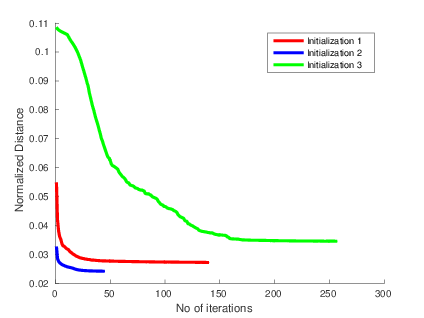
\epsfig{file=images/dist_change_euall.png,  width=0.5\textwidth}
\caption{The convergence of solution for \textbf{EUall} dataset. The number of iterations it took to converge differs for different initializations.}
\end{figure}

\begin{figure*}
\centering
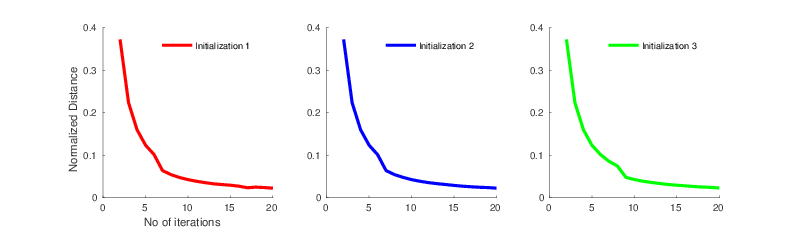
\epsfig{file=images/varying_k_distance.png,height=0.2\textheight, width=\textwidth}
\caption{The normalized distance of \textbf{facebook} dataset for different k ranging from 2 to 20.}
\end{figure*}

\begin{figure*}
\centering
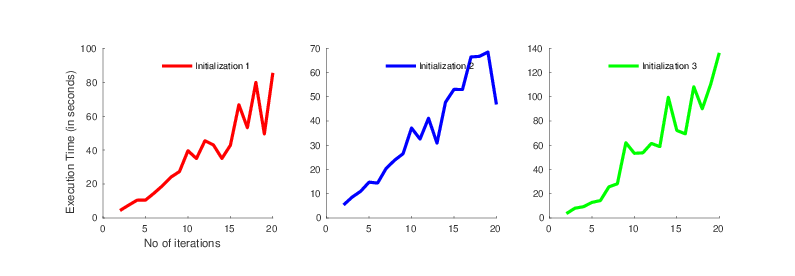
\epsfig{file=images/varying_k_time.png,height=0.2\textheight, width=\textwidth}
\caption{The execution time of \textbf{facebook} dataset for different k ranging from 2 to 20.}
\end{figure*}

\begin{figure}
\begin{tikzpicture}
\begin{axis}[xlabel={iteration $i$}, ylabel= {$\cost{\role_i} / \cost{\role'}$},
    height = 3.5cm,
    width = \columnwidth,
    cycle list name=yaf,
	yticklabel style={/pgf/number format/fixed},
	scaled ticks = false,
    %xmin = 1,
    %ymin = 0.2,
    %ymax = 1,
	ymin = 0.02,
	ytick = {0.02, 0.04, 0.06, 0.08, 0.1},
    xtick = {1, 51, 101, 151, 201, 251},
	legend entries = {\alginitrnd, \alginitdeg, \alginitone, \alginitkm}
    ]

\addplot+[no markers]
    table[x expr = {\coordindex + 1}, y index = 1, header = false]  {images/plot data/euall_init3.log};
\addplot+[no markers]
    table[x expr = {\coordindex + 1}, y index = 1, header = false]  {images/plot data/euall_init1.log};
\addplot+[no markers]
    table[x expr = {\coordindex + 1}, y index = 1, header = false]  {images/plot data/euall_init2.log};
\addplot+[no markers]
    table[x expr = {\coordindex + 1}, y index = 1, header = false]  {images/plot data/euall_init4.log};

\pgfplotsextra{\yafdrawaxis{1}{257}{0.02}{0.11}}
\end{axis}
\end{tikzpicture}
\caption{The convergence of solution for \EUall dataset. The cost of a role assignment $r_i$ at the end of $i$th iteration,
normalized by $\cost{r'}$ such that $r'(v) = 0$, for every $v$, that is, $r'$ assigns the same role to every vertex.}
\end{figure}
\fi

\section{Concluding remarks}
\label{sec:conclusions}

In this paper we propose a new type of role discovery optimization problem:
the vertices should have the same role if their profiles, role
counts of neighbors, are similar.

From technical point, our method is different than feature-based techniques
because our features are in fact roles of neighbors.
%Hence, a two-step
%approach---($i$) construct features and ($ii$) cluster roles from
%features---does not work.
This dependency makes the optimization
problem difficult: we show that the problem is \np-hard, and cannot be even approximated if we fix the
centroids for the roles.

On the positive side we show that we can discover the perfect, zero-cost,
solution with minimal number of roles efficiently in polynomial time. When the
number of roles is fixed, we propose two simple natural heuristics: iterative
optimization and a hill-climbing algorithm.

Interestingly enough, we do not directly use any network-based feature when
comparing vertices. Instead, we are only interested in role counts. Our logic
is that fundamentally different ego-networks for vertices, say, $u$ and $v$,
should result in different role counts which should imply that $u$ and $v$ are
different. Nevertheless, combining our approach with other feature-based role
discovery methods provides a potentially fruitful direction for future work. 


%
% The following two commands are all you need in the
% initial runs of your .tex file to
% produce the bibliography for the citations in your paper.

\bibliographystyle{IEEETran}
\bibliography{roles} 

\appendix

We will first prove Proposition~\ref{proposition:np}.

\begin{proof}[of Proposition~\ref{proposition:np}]
We will prove the hardness from \tmatch: an \np-hard problem where we are given
a universe $U$ and family $\mathcal{M}$ of sets of size $3$, and we are asked
to find a maximum disjoint cover. 

Assume that we are given an instance $(U, \mathcal{M})$ of \tmatch.  Let $n =
\abs{U}$ and $m = \abs{\mathcal{M}}$. We can safely assume that $n$ is divisible by 3.

Define $h = {n \choose 3}$ the number of possible
sets of size $3$ over $U$. Let $\ell = {n - 1 \choose 2}$ be the number of possible
sets of size $3$ containing a fixed vertex in $U$.
Let us define $t = 8m$ and $s = 2t$.

\emph{Graph construction:}
The graph constists of two major parts.

The first part entails 7 vertex sets: we start with $A_1$ and $A_2$ with $\abs{A_1} = 3$ and $\abs{A_2}
= \ell - 1$.
A single vertex, say $v$, 
is connected to an additional vertex, say $w$. We write $A_3 = \set{v}$ and $A_4 = \set{w}$.
Futhermore, $w$ is connected to a biclique of $A_5 = K(s, s)$.
%Each vertex $a \in A_1$ is connected to its own clique of size $h$; the vertices in these cliques form $A_6$.

Each vertex $u \in A_1$ and $v \in A_2$ is connected with a \emph{fat} edge:
$t$ copies of a path $u$--$x$--$v$, where $x$ is a vertex unique to the path.
These vertices form $A_6$.
Similarly, each vertex $u \in A_1$ and $v \in A_3$ is connected with a \emph{fat} edge;
the intermediate vertices form $A_7$.

%Finally, one
%vertex, say $b^* \in B$ is connected to an additional vertex, who is also connected
%to a biclique $K(s, s)$.

The final graph consists of $t$ copies of the first part. We redefine $A_i$ to be
the union of the corresponding groups in each copy.

The second part is very similar to the first.  It entails the vertex sets
$B_1$, $B_2$, and $B_3$ with $\abs{B_1} = n$, $\abs{B_2} = h - m$ $\abs{B_3} = m$.
Here $B_1$ corresponds to the universe $U$, and $B_2$ and $B_3$ correspond to
triplets of elements in $U$. Each vertex in $B_3$ is connected to its own vertex.
These vertices form $B_4$. Each vertex in $B_4$ is also connected to its own dedicated biclique
$K(s, s)$. The vertices in bicliques form $B_5$.
A vertex in $B_2$ is connected to the corresponding vertices in $B_1$ with a fat edge
of size $t$. The intermediate vertices form $B_6$.
Similarly, a vertex in $B_3$ is connected to the corresponding vertices in $B_1$ with a fat edge
of size $t$. The intermediate vertices form $B_7$.



\iffalse
The first part entails vertex sets $A$ and $B$ with $\abs{A} = 3$ and $\abs{B}
= \ell$.  Each vertex $a \in A$ and $b \in B$ is connected with a \emph{fat} edge:
$t$ copies of a path $a$--$x$--$b$, where $x$ is a vertex unique to the path.
Each vertex $a \in A$ is connected to its own clique of size $h$.  Finally, one
vertex, say $b^* \in B$ is connected to an additional vertex, who is also connected
to a biclique $K(s, s)$.

The final graph consists of $t$ copies of the first part.

The second part is very similar to the first.  It entails the vertex sets $A'$
and $B'$ with $\abs{A'} = n$ and $\abs{B'} = h$. Here $A'$ corresponds to the
universe $U$.  Each vertex $a \in A'$ and $b \in B'$ is connected with a
\emph{fat} edge of size $t$.  Finally, let $C'$ be the subset of $B'$ that
corresponds to the sets in $\mathcal{M}$.  Each vertex $c \in C'$ is connected
to its own unique vertex. We will denote these vertices by $O'$.
Each vertex in $O'$ is also connected to its own dedicated bi-clique
$K(s, s)$. 
\fi

\emph{Role assignment:}
Let us now define a role assignment, later this will turn out to be the optimal
assignment. Let $\mathcal{W}$, not necessarily a subset of $\mathcal{M}$, be a
matching covering completely $U$.

Let $C_3$ be the vertices in $B_2 \cup B_3$ corresponding to $\mathcal{W}$.
Let $C_1 = B_1$, $C_2 = (B_2 \cup B_3) \setminus C_3$ $C_4 = B_4$, $C_5 = B_5$.
Let $C_6$ be the vertices in $B_6 \cup B_7$ adjacent to $C_3$, and set $C_7 = (B_6 \cup B_7) \setminus C_6$.
We define $\role(v) = i$, where $v \in A_i \cup C_i$.
Let us write $\role_{\mathcal{W}} = \role$.

Let us compute the cost of $\role$.
To that end, write $c_{ij}$ to be the cost incurred by the $j$th component of the $i$th role.
The only non-zero costs are $c_{24}$, $c_{42}$, $c_{34}$, and $c_{43}$.
Define $n_i = \abs{\set{v ; \role(v) = i}}$,
and let $\alpha = \abs{A_3 \cup (B_3 \cap C_3)}$ and $\beta = \abs{B_3 \cap C_2}$.
We can express the cost as
\[
	c_{24} + c_{34} + c_{42} + c_{43} = f(\beta, n_2) + f(\alpha, n_3) + 2f(\alpha, n_4),
	%c_{24} = f(\beta, n_2)
	%c_{34} = f(\alpha, n_3)
	%c_{42} = f(\alpha, n_4)
\]
where $f(x, y) = x(y - x)/y$.
The counts $n_i$ do not depend on $\mathcal{W}$.
Since $\alpha + \beta = n_4$, so the cost of depends on $\mathcal{W}$ only via $\alpha$.
We have $2\alpha \geq 2t \geq n_3, n_4$ and $2\beta \leq 2m \leq t \leq n_2$.
Since $f(x, y)$ is a parabola peaking at $x = y / 2$,
the cost decreases as $\alpha$ increases.

Since $f(x, y) \leq \min(x, y / 2 - x)$, we can upper-bound the cost
by $n_3 + 2n_4 - 3\alpha + \beta < 4m$.

\iffalse

Let $\alpha = \abs{A_3 \cup C_3}$ be the number of vertices with $\role(v) = 3$.
Let $\beta = \abs{A_2 \cup C_2}$ be the number of vertices with $\role(v) = 2$.
Define also $\alpha_1 = \abs{A_3 \cup (B_3 \cap C_3)}$,
and $\beta_1 = \abs{B_3 \cap C_2}$.
A laborous comptuation reveals that the cost of $\role$ is equal to
\begin{equation}
\label{eq:cost}
	f(\alpha_1, \alpha) + f(\beta_1, \beta) + 2f(\alpha_1, \alpha_1 + \beta_1),
\end{equation}
where $f(x, y) = 2x(y - x)/y$.
Note that $\alpha$, $\beta$, and $\alpha_1 + \beta_1 = \abs{A_2} + \abs{B_3}$ are all constant.
Moreover, since
$\alpha_1 \geq \alpha / 2$,
$\beta_1 \leq \beta / 2$,
$\alpha_1 \geq \beta_1$, Eq.~\ref{eq:cost} decreases as $\abs{B_3 \cap C_3}$ increases.

Since $f(x, y) \geq x$ for $x \leq y / 2$,
we can upper-bound the cost by
\[
\begin{split}
	\alpha - \alpha_1 + \beta_1 + 2\beta_1 & = \abs{A_3 \cup C_3} - \abs{A_3 \cup (B_3 \cap C_3)} + 
	t + n / 3 - (t + \abs{D}) + 3(m - \abs{D}) \\
	& = n / 3 + 3m - 4\abs{D} < 4m.
\end{split}
\]

\emph{Role assignment:}
Let us now define a role assignment, this will turn out to be optimal
assignment.  Let $\mathcal{W} \subseteq \mathcal{U}$ be the maximum matching.
If $\mathcal{W}$ does not cover completely $\mathcal{U}$, then let $\mathcal{W}'$
be additional sets outside $\mathcal{M}$ completing the matching.
Let $D$ be the vertices in $B'$ corresponding to $\mathcal{W}$.
Let $D'$ be the vertices in $B'$ corresponding to $\mathcal{W}'$.
Let $K$ be the union of all bi-cliques.
\[
	\role(v) =
\begin{cases}
1 & v \in K,\\
2 & v \text{ adjacent to } K,\\
3 & v \in A \text{ or } v \in A',\\
4 & v \in D \cup D', \text{ or } v = b^*, \\
5 & v \in B' \setminus (D \cup D'), \text{ or } v \in B \setminus \set{b^*},\\
6 & v \text{ is a fat edge adjacent to } w, \role(w) = 4,\\
7 & v \text{ is a fat edge adjacent to } w, \role(w) = 5.\\
\end{cases}
\]

Define the roles as follows: The roles of vertices in bi-cliques $K(s, s)$ are
set to 2, the roles of adjacent vertices to the bi-cliques are set to 1. The
roles of vertices in $A$ and $A'$ are set to 3. The roles of vertices
corresponding to $\mathcal{W}$, as well as $b^*$, are set to $4$.
The roles for the remaining vertices in $B$ and $B'$ are set to 

Let us compute the cost of $\role$.
Let $\alpha = t + n / 3$ be the number of vertices with $\role(v) = 4$.
Among these vertices,
let $\alpha_1 = t + \abs{D}$ be the number of vertices adjacent to a vertex with
a role of 2.
Let $\beta = t\ell + k - \alpha$ be the number of vertices with $\role(v) = 5$.
Among these vertices,
let $\beta_1 = m - \abs{D}$ be the number of vertices adjacent to a vertex with
a role of 2.
A laborous comptuation reveals that the cost of $\role$ is equal to
\begin{equation}
\label{eq:cost}
	f(\alpha_1, \alpha) + f(\beta_1, \beta) + 2f(\alpha_1, \alpha_1 + \beta_1),
\end{equation}
where $f(x, y) = 2x(y - x)/y$. Note that $\alpha$, $\beta$, and $\alpha_1 + \beta_1$ are all constant.
Moreover, since
$\alpha_1 \geq \alpha / 2$,
$\beta_1 \leq \alpha / 2$,
$\alpha_1 \geq \beta$, Eq.~\ref{eq:cost} decreases as $\abs{D}$ increases.


Since $f(x, y) \geq x$ for $x \leq y / 2$,
we can upper-bound the cost by
\[
\begin{split}
	\alpha - \alpha_1 + \beta_1 + 2\beta_1 & = t + n / 3 - (t + \abs{D}) + 3(m - \abs{D}) \\
	& = n / 3 + 3m - 4\abs{D} < 4m.
\end{split}
\]

\fi

\emph{Role $\role$ is optimal:}
Let $\role^*$ be the optimal role assignment with a cost of $\sigma$.  Consider
that if instead of selecting optimal centroids for $\role^*$, we select the
optimal centroids---we denote them by $\mu'$---among the profiles of the
vertices in the cluster. We know that the cost of $\role^*$ w.r.t. $\mu'$, say
$\tau$, is at most $2\sigma$. If $\tau \geq 8m$, then $\sigma \geq 4m$, the cost of $\role$, which
violates the optimality of $\role^*$. Consequently, $\tau < 8m = t$.

Note that $\mu'$ are all integral. We can safely assume that the copies of the
first part of the graph have the same role assignment. This immediately implies
that the profiles of $\role^*$ should match \emph{exactly} the centroids $\mu'$.

There are 6 groups with distinct degrees in the first part:
$\dg{u} = t\ell$ for $u \in A_1$,
$\dg{u} = 3t$ for $u \in A_2$,
$\dg{u} = 1 + 3t$ for $u \in A_3$,
$\dg{u} = 2s + 1$ for $u \in A_4$,
$\dg{u} = s + 1$ for $u \in A_5$,
$\dg{u} = 2$ for $u \in A_6 \cup A_7$.
Since the vertices from different groups have different degrees, $\role^*$
must be a refinement of this partition.
Moreover, $A_6$ connects to $A_2$ and $A_7$ connects to $A_3$.
Thus they cannot have the same role. 
This gives us 7 groups, and $\role^*$ must be a refinement of this partition.
Since we have only 7 roles, this must be the role assignment.

Let us now consider the second part of the graph.
Let $u \in B_1$.
The only integral centroid that matches $\dg{u}$ is $\mu'_1$, and the
remaining centroids differ in degree
by at least of $t$, consequently $\dist{u, \mu'_i} \geq t$ for $i \neq 3$.
This forces, $\role^*(u) = 1$. Similarly,
$\role^*(u) = 4$, for $u \in B_4$, 
$\role^*(u) = 5$, for $u \in B_5$,
$\role^*(u) = 6, 7$, for $u \in B_6 \cup B_7$.

Let $u \in B_2 \cup B_3$. If $\role^*(u) \neq 2, 3$, then each vertex in a fat edge will
introduce a cost of at least 1, when compared to the integral centroids $\mu'$.
Since there are $t$ of these vertices, we must have $\role^*(u) = 2, 3$.  Using
a similar argument, among the vertices in $B_2 \cup B_3$ adjacent (by a fat edge) to a vertex $v \in B_1$,
only one has the role $3$, the remaining adjacent vertices have the role $2$.

This shows that $\role^* = \role_{\mathcal{W}}$, where $\mathcal{W}$ are the sets corresponding
to the vertices with role $3$. We saw earlier that the cost is minimized when $\alpha = t +
\abs{\mathcal{W} \cap \mathcal{M}}$
is maximized.
\end{proof}


\iffalse
\emph{(i)} a vertex $o$ with $\dg{o} = 2s + 1$,
\emph{(ii)} a vertex in $K(s, s)$ with $\dg{o} = s + 1$,
\emph{(iii)} vertices $a \in A$ with $\dg{a} = t\ell$,
\emph{(iv)} vertex $b^*$ with $\dg{b^*} = 1 + 3t$,
\emph{(v)} the remaining vertices $b \in B \setminus \set{b^*}$ with $\dg{b} = 3t$, and finally
\emph{(vi)} the vertices in fat edges with degree of $2$.
Since the vertices from different groups have different degrees, $\role^*$
must be a refinement of this partition. Note that the fat edges can be split further into
two groups:
\emph{(vi.a)} vertices connecting to $b^*$, and
\emph{(vi.b)} vertices connecting to $B \setminus \set{b^*}$.
This gives us 7 groups, and $\role^*$ must be a refinement of this partition.
Since we have only 7 roles, this must be the role assignment.


Let us now consider the second part of the graph.
Let $a \in A'$.
The only integral centroid that matches $\dg{a}$ is $\mu'_3$, and the
remaining centroids differ in degree
by at least of $t$, consequently $\dist{a, \mu'_i} \geq t$ for $i \neq 3$.
This forces, $\role^*(a) = 3$. Similarly, each vertex $o \in O'$ has
$\role^*(o) = 1$, and the vertices in the bi-cliques have the role 2.
Each vertex $x$ in a fat edge must have $\role^*(x) = 6$ or $\role^*(x) = 7$.

Let $b \in B'$. If $\role^*(b) \neq 4, 5$, then each vertex in a fat edge will
introduce a cost of at least 1, when compared to the integral centroids $\mu'$.
Since there are $t$ of these vertices, we must have $\role^*(b) = 3, 4$.  Using
a similar argument, among the vertices in $B'$ adjacent to a vertex $a \in A'$,
only one has the role $4$, the remaining adjacent vertices have the role $5$.


The cost of $\role^*$ is now lower-bounded by the cost given in
Eq.~\ref{eq:cost}, and it is equal if and only if $\role^* = \role$.

Since the cost of $\role$ decreases as $\abs{D}$ increases, the optimal $\role$
will correspond to the optimal matching.
\end{proof}
\fi

To prove Proposition~\ref{proposition:np-fixed},
we need to introduce the following \np-complete problem.

\begin{problem}[\tuples]
Assume a universe $U$ and a set $\mathcal{S}$ of 5-tuples over $U$,
such that each $u \in U$ occurs in at least 3 tuples.
Is there a subset $B \subseteq U$ such that each exactly 2 entries in each $S \in \mathcal{S}$
belong to $B$.
\end{problem}

\begin{proposition}
\tuples is \np-complete.
\end{proposition}

\begin{proof}
\tuples is obviously in \np. We prove the hardness by reduction from \tsat.

Assume that we are given $m$ clauses $C_1, \ldots, C_m$ using $n$ variables, in
total. We can safely assume that each clause contains exactly 3 variables by
allowing the repetition of a variable.

We define the universe $U$ to contain $2n + 2 + 2m$ variables, which we will
denote by $t$, $f$, $x_1, \ldots, x_n$, $y_1, \ldots, y_n$,
$d_1, \ldots, d_m$, and $e_1, \ldots, e_m$.
To simplify notation,
we will identify $x_i$ with the $i$th positive literal and $y_i$ with the $i$th negative literal. 

We introduce the following clauses:
\emph{(1)} $(t, t, f, f, f)$,
\emph{(2)} $(x_i, \neg x_i, t, f, f)$, where $i = 1, \ldots, n$,
\emph{(3)}
$(\neg c_1, \neg c_2, \neg c_3, d_j, e_j)$, where $C_j = c_{1} \lor c_{2} \lor c_{3}$
is the $j$th clause.

To make sure that each variable occurs in at least 3 tuples, we copy each tuple
3 times.


Assume there is $B$ solving \tuples. Set the $i$th variable to be true if $x_i \in B$, and false otherwise.
At most $2$ variables $\neg c_i$ are in $B$, for $C_j = c_{1} \lor c_{2} \lor c_{3}$.
Assume that $\neq c_1 = \notin B$.
Since either $x_i \in B$ or $\neg x_i \in B$, this forces $c_1 \in B$, 
making $C_j$ satisfied.

Now assume that we can satisfy each clause. First set $B = \set{t}$. Add
$x_i$ into $B$ if the $i$th variable is true, otherwise insert $\neg x_i$.
Since a clause $C_j = c_{1} \lor c_{2} \lor c_{3}$ is satisfied, we have at most 2 entries in $B$ among $\neg c_i$. 
Insert $d_j$ and/or $e_j$ to $B$ so that $(\neg c_1, \neg c_2, \neg c_3, d_j, e_j)$ contains exactly 2 entries in $B$.
The resulting $B$ solves \tuples.
\end{proof}

\begin{proof}[of Proposition~\ref{proposition:np-fixed}]
The problem is in \np.  We will prove the hardness from \tuples.
Assume that we are given an instance $(U, \mathcal{S})$ of \tuples.
Let $n = \abs{U}$ and $m = \abs{\mathcal{S}}$.
Let $\ell_u$ be the total number of occurrences, counting multiplicities,
of $u$ in $\mathcal{S}$.

Define the graph as follows:
For each $u \in U$, add a cycle of length $\ell_u$. Note that the cycle is simple
since $\ell_u \geq 3$. Denote this cycle by $D_u$.

For each tuple $C_j$ add a vertex $w_j$, and connect it to 
a vertex in $D_u$, where $u \in C_j$. The connection can and should be done such
that each vertex in each cycle is connected to exactly one $w_j$.

Set the number of roles $k = 3$, and define the following centroids $\mu_1 = (2, 0, 1)$, $\mu_2 = (0, 2, 1)$,
and $\mu_3 = (2, 3, 0)$.

Let $r$ be the optimal role assignment for the defined centroids.
The cost of is 0 if and only if
\emph{(i)} every vertex in $v \in D_u$ has the same role, $\role(v) = 1, 2$,
\emph{(ii)} $\role(w_j) = 3$,
\emph{(iii)} for each $w_j$ there are two adjacent vertices with role 1
and three adjacent vertices with role 2.

Consequently, $B$ in \tuples corresponds to the vertices with role 1.
\end{proof}


\end{document}
